\documentclass[10pt,draft]{article}

\usepackage{mylhs2tex}
\usepackage{amsmath}
\usepackage{amssymb}
\usepackage{amsthm}
\usepackage{paralist}
\usepackage[final,hidelinks]{hyperref}
\usepackage{tabularx}
\usepackage{bussproofs}
\usepackage[final]{listings}
\usepackage{stmaryrd}
\usepackage{cases}
\usepackage{mathtools}
\usepackage{multicol}
\usepackage{url}
\urlstyle{sf}
\usepackage[usenames,dvipsnames]{color}
\usepackage{tikz}
\usetikzlibrary{calc}
\usetikzlibrary{shapes}
\usetikzlibrary{positioning}
\usepackage{textcomp}
\usepackage{ifdraft}
\usepackage{xspace}

\theoremstyle{plain}
\newtheorem{theorem}{Theorem}[section]
\newtheorem{lemma}[theorem]{Lemma}
\newtheorem{proposition}[theorem]{Proposition}
\newtheorem{corollary}[theorem]{Corollary}
\newtheorem{observation}[theorem]{Observation}
\theoremstyle{definition}
\newtheorem{definition}[theorem]{Definition}
\newtheorem{example}[theorem]{Example}
\newtheorem{remark}[theorem]{Remark}

% DSL keywords
\newcommand{\keyword}[1]{\ensuremath{\mathbf{#1}}}
\newcommand{\recordname}[1]{\ensuremath{\mathsf{#1}}}
\newcommand{\fieldname}[1]{\ensuremath{\mathsf{#1}}}

% Types
\newcommand{\tbool}{\keyword{Bool}}
\newcommand{\tchar}{\keyword{Char}}
\newcommand{\tint}{\keyword{Int}}
\newcommand{\treal}{\keyword{Real}}
\newcommand{\tstring}{\keyword{String}}
\newcommand{\ttimestamp}{\keyword{Timestamp}}
\newcommand{\tduration}{\keyword{Duration}}
\newcommand{\tdt}{\keyword{DurationTimestamp}}
\newcommand{\tlist}[1]{\ensuremath{\left[#1\right]}}
\newcommand{\tent}[1]{\ensuremath{\left\langle#1\right\rangle}}
\newcommand{\subrec}{\le}
\newcommand{\closure}[1]{\mathrm{Cl}\left(#1\right)}

% Domains
\newcommand{\drecordname}{\mathit{RecordName}}
\newcommand{\dfieldname}{\mathit{FieldName}}
\newcommand{\dvalue}{\mathit{Value}}
\newcommand{\dbool}{\mathit{Bool}}
\newcommand{\dint}{\mathit{Int}}
\newcommand{\dreal}{\mathit{Real}}
\newcommand{\dstring}{\mathit{String}}
\newcommand{\dtimestamp}{\mathit{Timestamp}}
\newcommand{\dduration}{\mathit{Duration}}
\newcommand{\drecord}{\mathit{Record}}
\newcommand{\dlist}{\mathit{List}}
\newcommand{\dent}{\mathit{Ent}}
\newcommand{\dfields}{\mathit{Fields}}
\newcommand{\dchar}{\mathit{Char}}
\newcommand{\dstore}{\mathit{Store}}
\newcommand{\dtype}{\mathit{Type}}
\newcommand{\entlookup}{\operatorname{lookup}}

\newcommand\depend{\rightarrow}
\newcommand{\finmap}{\rightharpoonup_{\mathrm{fin}}}
\newcommand{\parto}{\rightharpoonup}
\newcommand{\dom}[1]{\operatorname{dom}(#1)}
\newcommand{\rem}[2]{\operatorname{rem}(#1,#2)}
\newcommand{\powerset}{\mathcal{P}}
\newcommand{\powersetfin}{\powerset_{\mathrm{fin}}}
\newcommand{\muerp}{$\mu$ERP\xspace}

% Type system
\newcommand{\hastype}[4]{#1, #2 \vdash #3 : #4}
\newcommand{\issubtype}[3]{#1 \vdash #2 <: #3}
\newcommand{\constrEnt}[3]{#1, #2 \Vdash #3}
\newcommand{\reptype}[5]{#1, #2, #3 \vdash #4 : #5}

% Ontology
\newcommand{\ontden}[1]{\left\llbracket #1 \right\rrbracket}
\newcommand{\ontdentp}[1]{\left\llbracket #1 \right\rrbracket}

% Environment for writing BNF grammars
\newcolumntype{R}{>{\raggedleft\arraybackslash}X}
\newenvironment{bnf}{\setlength{\tabcolsep}{2pt}\noindent\tabularx{\textwidth}{>{$\it
    }l<{$}>{$}r<{$}>{$\it }l<{$}R}}{\endtabularx}
\newcommand\ebnf{::=}
\newcommand{\bnfsep}{\mid}

% Parrot
\newcommand\derefCxt{@}
\newcommand\derefNow{!}
\newcommand\image[1]{\mathsf{Im}(#1)}
\newcommand\natseg[1]{\left[#1\right]}
\newcommand\step{\rightarrow}
\newcommand\ecxt{{\mathbb E}}
\newcommand\fcxt{{\mathbb F}}
\newcommand\eapp[1]{{\mathbb E}\left[#1\right]}
\newcommand\fapp[1]{{\mathbb F}\left[#1\right]}
\newcommand\cxthole{\left[\cdot\right]}
\newcommand\strict[1]{\mathsf{strict}(#1)}
\newcommand\nstrict[1]{\ob{\mathsf{strict}}(#1)}
\newcommand\infrule[2]{ %
  \RightLabel{(#1)}%
  \AxiomC{\phantom{FOOBAR}}%
  \UnaryInfC{$#2$}%
  \DisplayProof{}%
}%
\newcommand\infruleI[3]{%
  \RightLabel{(#1)}%
  \AxiomC{$#2$}%
  \UnaryInfC{$#3$}%
  \DisplayProof{}%
}
\newcommand\infruleII[4]{%
  \RightLabel{(#1)}%
  \AxiomC{$#2$}%
  \AxiomC{$#3$}%
  \BinaryInfC{$#4$}%
  \DisplayProof{}%
}

\newcommand\infruleIII[5]{%
  \RightLabel{(#1)}%
  \AxiomC{$#2$}%
  \AxiomC{$#3$}%
  \AxiomC{$#4$}%
  \TrinaryInfC{$#5$}%
  \DisplayProof{}%
}

\newcommand\arity[1]{\mathsf{ar}(#1)}
\newcommand\vdur[1]{\langle\langle#1\rangle\rangle}
\newcommand\vdate[1]{\langle\langle#1\rangle\rangle}
\newcommand\dminus{\ensuremath{\mathop{\langle-\rangle}}}
\newcommand\dplus{\ensuremath{\mathop{\langle+\rangle}}}
\newcommand{\vlist}[1]{\ensuremath{\left[#1\right]}}
\newcommand{\valref}[1]{\ensuremath{\left\langle#1\right\rangle}}
\newcommand\calC{{\mathcal C}}
\newcommand\calD{{\mathcal D}}
\newcommand\calR{{\mathcal R}}
\newcommand\calE{{\mathcal E}}
\newcommand{\set}[1]{\left\{#1\right\}}
\newcommand\letin[2]{\keyword{let}\;#1\;\keyword{in}\;#2}
\newcommand\equals{=}
\newcommand\typeof[2]{\keyword{type}\;#1\;\keyword{of}\;#2}
\newcommand\semi{;}
\newcommand\default{\_}
\newcommand\block[1]{\left\{#1\right\}}
\newcommand\constr[2]{#1\Vdash #2}
\newcommand\constrt[1]{\constr{}{#1}}
\newcommand\type[4]{#1; #2\vdash #3 : #4}
\newcommand\foldr{\keyword{fold}}
\newcommand\cons{\mathop{\#}}
\newcommand\ifelse[3]{\keyword{if}\;#1\;\keyword{then}\;#2\;\keyword{else}\;#3}
\newcommand\subst[3]{#1\substitution{\repl{#2}{#3}}}
\newcommand\substitution[1]{\left[#1\right]}
\newcommand\repl[2]{#1/#2}

\newcommand\ordC[1]{\mathsf{Ord}(#1)}
\newcommand\eqC[1]{\mathsf{Eq}(#1)}
\newcommand\implC{\Rightarrow}
\newcommand\fieldC[3]{#1.#2:#3}
\newcommand\tup[1]{\overline{#1}}
\newcommand\seq[1]{\left\langle #1 \right\rangle}
\newcommand\emptyseq{\seq{}}
\newcommand\fv[1]{\mathsf{fv}(#1)}
\newcommand\mhole{\_}


\newcommand\nats{{\mathbb N}}
\newcommand\reals{{\mathbb R}}
\newcommand\ctrue{\mathbf{True}}
\newcommand\cfalse{\mathbf{False}}

\newcommand\trule[3]{\begin{gathered}\inferrule*{#2}{#3}
    \tag{#1}\end{gathered}}
\newcommand{\prt}[1]{\lstinline[language=parrot,basicstyle=\normalsize]!#1!}
\newcommand{\prtalt}[1]{\lstinline[language=parrot,basicstyle=\normalsize]|#1|}
\newcounter{dummycounter}
\newcommand{\lstinputreport}[2]{%
  \setcounter{dummycounter}{#1}%
  \lstinputlisting[language=parrotprelude,xleftmargin=0pt,lastline=\arabic{dummycounter},belowskip=0pt]{#2}%
  \stepcounter{dummycounter}%
  \lstinputlisting[language=parrot,xleftmargin=0pt,firstline=\arabic{dummycounter}]{#2}}
\newcommand{\lstinputintreport}[2]{\paragraph{#2}

~

\lstinputreport{#1}{muERP/reporting/System/#2.rep}}
\newcommand{\lstinputextreport}[2]{\paragraph{#2}

~

\lstinputreport{#1}{muERP/reporting/#2.rep}}

%PCSL
\newcommand{\pcsl}[1]{\lstinline[language=pcsl,basicstyle=\normalsize]!#1!}

% Macro for identifiers in POETS DSLs
\makeatletter
\newcommand*\poetsidstyle{\expandafter\id@style\the\lst@token\relax}
\def\id@style#1#2\relax{%
        \ifcat#1\relax\else
                \ifnum`#1=\uccode`#1%
                        \sffamily
                \else
                        \itshape
                \fi
        \fi
}
\makeatother

\lstdefinelanguage{ontology}
{
 xleftmargin=\parindent,
 basicstyle=\upshape\scriptsize,
 keywordstyle=\bfseries,
 identifierstyle=\itshape,
 commentstyle=\itshape\bfseries,
 sensitive=true,
 keepspaces=true,
 columns=fullflexible,
 mathescape=true,
 showstringspaces=false,
 comment=[l]\#
}

\lstdefinelanguage{pcsl}
{
 xleftmargin=\parindent,
 basicstyle=\upshape\scriptsize,
 keywordstyle=[1]\bfseries,
 keywordstyle=[2]\itshape,
 identifierstyle=\poetsidstyle,
 commentstyle=\itshape\bfseries,
 stringstyle=\ttfamily,
 sensitive=true,
 keepspaces=true,
 columns=fullflexible,
 mathescape=true,
 showstringspaces=false,
 comment=[l]//,
 string=[b]{"},
 keywords=[1]{name,type,description,contract,clause,val,fun,fulfilment,%
                   where,due,within,after,%
                   immediately,remaining,if,then,else,when,case,of,and,or,let,%
                   in,Bool,Int,Double,String,Timestamp,Duration},
 morekeywords=[2]{S,m,H,D,W,M,Y},
 literate=*{<}{$\langle$}{1} {>}{$\rangle$}{1} {->}{$\rightarrow$}{1}
                {\\}{$\lambda$}{1}
                {*}{$\times$}{1}
                {<=}{$\le$}{1} {>=}{$\ge$}{1}
                {==}{$\equiv$}{1} {/=}{$\not\equiv$}{1}
                {&&}{$\land$}{1}
                {||}{$\lor$}{1}
                {not}{$\lnot$}{1}
                {<+>}{$\langle + \rangle$}{3}
                {<->}{$\langle - \rangle$}{3}
                {<*>}{$\langle \times \rangle$}{3}
                {\ <\ }{\ $<$\ }{3} {\ >\ }{\ $>$\ }{3}
}

\lstdefinelanguage{parrot}
{
 xleftmargin=\parindent,
 basicstyle=\upshape\scriptsize,
 keywordstyle=\bfseries,
 identifierstyle=\poetsidstyle,
 commentstyle=\itshape\bfseries,
 stringstyle=\ttfamily,
 sensitive=true,
 keepspaces=true,
 columns=fullflexible,
 mathescape=true,
 showstringspaces=false,
 comment=[l]--,
 string=[b]{"},
 keywords={report,fold,Inl,Inr,True,False,if,then,else,let,in,%
                   type,reftype,of,pic,not,events,error,_,Bool,Int,Double,Char,String,%
                   Timestamp,Duration,Ord},
 literate=*{<}{$\langle$}{1} {>}{$\rangle$}{1} {->}{$\rightarrow$}{1}
                {<-}{$\leftarrow$}{1}
                {=>}{$\Rightarrow$}{1}
                {\\}{$\lambda$}{1}
                {*}{$\times$}{1}
                {<=}{$\le$}{1} {>=}{$\ge$}{1}
                {==}{$\equiv$}{1} {/=}{$\not\equiv$}{1}
                {&&}{$\land$}{1}
                {||}{$\lor$}{1}
                {not}{$\lnot$}{1}
                {<+>}{$\langle + \rangle$}{3}
                {<->}{$\langle - \rangle$}{3}
                {<*>}{$\langle \times \rangle$}{3}
                {\ <\ }{\ $<$\ }{3} {\ >\ }{\ $>$\ }{3}
                {++}{$+\hspace{-3pt}+$}{1}
}

\lstdefinelanguage{parrotprelude}
{
 xleftmargin=\parindent,
 basicstyle=\upshape\scriptsize,
 keywordstyle=\bfseries,
 identifierstyle=\itshape,
 sensitive=true,
 keepspaces=true,
 columns=fullflexible,
 mathescape=true,
 showstringspaces=false,
 keywords={name,description,tags}
}

\lstdefinelanguage{eventlog}
{
 xleftmargin=\parindent,
 basicstyle=\upshape,
 identifierstyle=\sffamily,
 commentstyle=\itshape\bfseries,
 stringstyle=\ttfamily,
 sensitive=true,
 keepspaces=true,
 columns=fullflexible,
 mathescape=true,
 showstringspaces=false,
 comment=[l]//,
 string=[b]{"},
 literate=*{<}{$\langle$}{1} {>}{$\rangle$}{1} {->}{$\rightarrow$}{1}
                {\\}{$\lambda$}{1}
                {*}{$\times$}{1}
                {<=}{$\le$}{1} {>=}{$\ge$}{1}
                {==}{$\equiv$}{1} {/=}{$\not\equiv$}{1}
                {&&}{$\land$}{1}
                {||}{$\lor$}{1}
                {not}{$\lnot$}{1}
                {<+>}{$\langle + \rangle$}{3}
                {<->}{$\langle - \rangle$}{3}
                {<*>}{$\langle \times \rangle$}{3}
                {\ <\ }{\ $<$\ }{3} {\ >\ }{\ $>$\ }{3}
}

\lstdefinelanguage{lithaskell}[]{haskell}{
 basicstyle=\ttfamily,
 flexiblecolumns=false,
 basewidth={0.5em,0.45em},
 literate={+}{{$+$}}1 {/}{{$/$}}1 {*}{{$*$}}1 {=}{{$=$}}1
          {>}{{$>$}}1 {<}{{$<$}}1 {\\}{{$\lambda$}}1
          {\\\\}{{\char`\\\char`\\}}1
          {->}{{$\rightarrow$}}2 {>=}{{$\ge$}}2 {<-}{{$\leftarrow$}}2
          {<=}{{$\le$}}2 {=>}{{$\Rightarrow$}}2
%          {\ .}{{$\circ$}}2 {\ .\ }{{$\circ$}}2
          {>>}{{>>}}2 {>>=}{{>>=}}2
          {|}{{$\mid$}}1}

\newcommand\maybecolor[1]{\ifdraft{\color{#1}}{}}
\newcommand{\displaycomment}[1]{\ifdraft{#1{}}{}}

\definecolor{dkgreen}{rgb}{0,0.4,0}

% The first parameter is the note author
% Active comments: something has to be done
\newcommand{\TODO}[2]{\displaycomment{{\maybecolor{red}{\bf #1: }{{\maybecolor{blue}#2}}}}}
% Things to keep in mind, potentially useful but no need to edit
\newcommand{\Remark}[2]{\displaycomment{{\maybecolor{dkgreen} {\bf
        #1:} #2}}}

\newcommand{\JA}[1]{\TODO{Jesper}{#1}}
\newcommand{\ja}[1]{\Remark{Jesper}{#1}}
\newcommand{\PB}[1]{\TODO{Patrick}{#1}}
\newcommand{\pb}[1]{\Remark{Patrick}{#1}}
\newcommand{\TOM}[1]{\TODO{Tom}{#1}}
\newcommand{\tom}[1]{\Remark{Tom}{#1}}

%%% Local Variables: 
%%% mode: latex
%%% TeX-master: "tr"
%%% End: 


\begin{document}
\title{Domain-Specific Languages for Enterprise Systems}
\author{Tom Hvitved \and Patrick Bahr \and Jesper Andersen}

% hack:
\renewcommand{\today}{\small Department of Computer Science, University of
    Copenhagen\\ Universitetsparken 1, 2100 Copenhagen, Denmark\\
  \{\texttt{hvitved,bahr,jespera}\}\texttt{@diku.dk}}

\maketitle

\begin{abstract}
  The process-oriented event-driven transaction systems (POETS)
  architecture introduced by Henglein et al. is a novel software architecture for
  enterprise resource planning (ERP) systems. POETS employs a pragmatic
  separation between
  \begin{inparaenum}[(i)]
  \item transactional data, that is what has happened;
  \item reports, that is what can be derived from the transactional
    data; and
  \item contracts, that is which transactions are expected in the
    future.
  \end{inparaenum}
  Moreover, POETS applies domain-specific languages (DSLs) for
  specifying reports and contracts, in order to enable succinct
  declarative specifications as well as rapid adaptability and
  customisation. In this report we document an implementation of a
  generalised and extended variant of the POETS architecture. The
  generalisation is manifested in a detachment from the ERP domain,
  which is rather an instantiation of the system than a built-in
  assumption. The extensions amount to a customisable data model based
  on nominal subtyping; support for run-time changes to the data
  model, reports and contracts, while retaining full
  auditability; and support for referable data that may evolve over
  time, also while retaining full auditability as well as referential
  integrity. Besides the revised architecture, we present the DSLs
  used to specify data definitions, 
  reports, and contracts respectively, and we provide the complete
  specification for a use case scenario, which demonstrates the
  conciseness and validity of our approach. Lastly, we describe
  technical aspects of our implementation, with focus on the techniques
  used to implement the tightly coupled DSLs.
\end{abstract}

\tableofcontents

\section{Introduction}
\label{sec:introduction}
Enterprise resource planning (ERP) systems are comprehensive software
systems used to manage daily activities in enterprises. Such
activities include---but are not limited to---financial management
(accounting), production planning, supply chain management and
customer relationship management. ERP systems emerged as a remedy to
heterogeneous systems, in which data and functionality are spread
out---and duplicated---amongst dedicated subsystems. Instead, an ERP
system it built around a central database, which stores all
information in one place.

Traditional ERP systems such as
Microsoft Dynamics
NAV\footnote{\url{http://www.microsoft.com/en-us/dynamics/products/nav-overview.aspx}.},
Microsoft Dynamics
AX\footnote{\url{http://www.microsoft.com/en-us/dynamics/products/ax-overview.aspx}.}, and
SAP\footnote{\url{http://www.sap.com}.}
are three-tier architectures with a client, an application
server, and a centralised relational database system. The central database
stores information in tables, and the application server provides the
business logic, typically coded in a general purpose, imperative
programming language. A shortcoming to this approach is
that the state of the system is decoupled from the business logic,
which means that business processes---that is, the daily
activities---are not represented explicitly in the system. Rather,
business processes are encoded implicitly as transition systems, where
the state is maintained by tables in the database, and transitions are
encoded in the application server, possibly spread out across several
different logical modules.

The process-oriented event-driven transaction systems (POETS)
architecture introduced by Henglein et al.~\cite{henglein09jlap} is a
qualitatively different approach to ERP systems. Rather than storing
both transactional data and implicit process state in a database,
POETS employs a pragmatic separation between transactional data, which
is persisted in an \emph{event log}, and \emph{contracts}, which are
explicit representations of business processes, stored in a separate
module. Moreover, rather than using general purpose programming
languages to specify business processes, POETS utilises a declarative
domain-specific language (DSL)~\cite{andersen06sttt}. The use of a DSL
not only enables explicit formalisation of business processes, it also
minimises the gap between requirements and a running system. In fact,
Henglein et al. take it as a goal of POETS that ``[...] the formalized
requirements \emph{are} the system''  \cite[page 382]{henglein09jlap}.

The bird's-eye view of the POETS architecture is presented in
Figure~\ref{fig:origArch}.
\begin{figure}[t]
  \centering\small
  \newcommand\drawInner[2]{
  \node[anchor=east,align=center] (t) at (#2.east) {#1};%
  \draw[thick] (t.north west) -- (t.north east)%
            (t.south west) -- (t.south east);%
  }
\newcommand\drawHeader[2]{
  \node[anchor=north] at (#2.north) {#1};
}
\newcommand\drawList[2]{
  \node[fill=white,draw,align=left] at (#2.south) {#1};
}

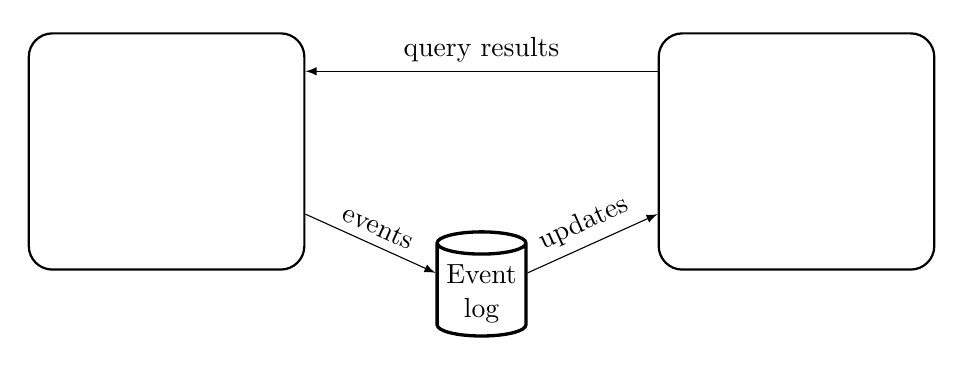
\begin{tikzpicture}
  [box/.style={shape=rectangle,rounded corners=3mm,minimum height=3cm,
    minimum width=3.5cm, anchor=north,draw},%
  db/.style={very thick,shape=cylinder, shape border
    rotate=90,aspect=.25,draw,align=center},%
  node distance=8cm]%
  \node[thick,box] (contract) {};%
  \drawHeader{Contract engine}{contract}%
  \drawInner{Running\\contracts}{contract}%
  \drawList{start contract\\register event\\end contract}{contract}%

  \node[thick,box,right of=contract] (report) {};%
  \drawHeader{Report engine}{report}%
  \drawInner{Report\\definitions}{report}%
  \drawList{add report\\delete report\\get report\\query report}{report}%

  \node[db,anchor=north] (events) at ($(contract)!.5!(report)-(0,1)$) {Event\\log};%

  \draw[-latex] (contract) edge[]
  node[above,midway,sloped] {events} (events)%
  (events) edge[] node[above,midway,sloped]
  {updates} (report)%
  (report.150) -- node[above,midway] {query results} (contract.30);%
\end{tikzpicture}
%%% Local Variables: 
%%% mode: latex
%%% TeX-master: "tr"
%%% End: 

  \caption{Bird's-eye view of the POETS
    architecture (diagram copied from~\cite{henglein09jlap}).}
  \label{fig:origArch}
\end{figure}
At the heart of the system is the event log, which is an append-only
list of transactions. Transactions represent ``things that take
place'' such as a payment by a customer, a delivery of goods by a
shipping agency, or a movement of items in an inventory. The
append-only restriction serves two purposes. First, it is a legal
requirement in ERP systems that transactions, which are relevant for
auditing, are retained. Second, the report engine utilises
monotonicity of the event log for optimisation, as shown by Nissen and
Larsen~\cite{nissen07ifl}.

Whereas the event log stores historical data, contracts play the role
of describing which events are expected in the future. For instance, a
yearly payment of value-added tax (VAT) to the tax authorities is an
example of a (recurring) business process. The amount to be paid to
the tax authorities depends, of course, on the financial transactions
that have taken place. Therefore, information has to be derived from
previous transactions in the event log, which is realised as a
\emph{report}. A report provides structured data derived from the
transactions in the event log. Like contracts, reports are written in
a declarative domain-specific language---not only in order to minimise
the semantic gap between requirements and the running system, but also
in order to perform automatic optimisations.

Besides the radically different software architecture, POETS
distinguishes itself from existing ERP systems by abandoning
the double-entry bookkeeping (DEB) accounting
principle~\cite{weygandt04book} in favour of the resources, events,
and agents (REA) accounting model of McCarthy~\cite{mccarthy82tar}.

In double-entry bookkeeping, each transaction is recorded as two
postings in a \emph{ledger}---a \emph{debit} and a
\emph{credit}. When, for instance, a customer pays an amount $x$ to
a company, then a debit of $x$ is posted in a cash account, and a
credit of $x$ is posted in a sales account, which reflects the flow of
cash from the customer to the company. The central invariant of DEB
is that the total credit equals the total debit---if not,
resources have either vanished or spontaneously appeared. DEB fits
naturally in the relational database oriented architectures, since
each ledger is similar in structure to a table. Moreover, DEB is the
de facto standard accounting method, and therefore used by
current ERP systems.

In REA, transactions are not registered in accounts, but rather as the
events that take place. An event in REA is of the form $(a_1,a_2,r)$
meaning that agent $a_1$ transfers resource $r$ to agent $a_2$. Hence,
when a customer pays an amount $x$ to a company, then it is
represented by a single event
$(\mbox{customer},\mbox{company},x)$. Since events are atomic, REA
does not have the same redundancy\footnote{In traditional DEB,
  redundancy is a feature to check for consistency. However,
  in a computer system such redundancy is superfluous.} as DEB, and
inconsistency is not a possibility: resources always have an origin and a
destination.  The POETS architecture not only fits with the REA
ontology, it is based on it. Events are stored as first-class objects
in the event log, and contracts describe the expected future flow of
resources.\footnote{Structured contracts are not part of the original
  REA ontology but instead due to Andersen et
  al.~\cite{andersen06sttt}.} Reports enable computation of derived 
information that is inherent in DEB, and which may be a legal
requirement for auditing. For instance, a sales account---which
summarises (pending) sales payments---can be reconstructed from
information about initiated sales and payments made by customers. Such
a computation will yield the same \emph{derived} information as in
DEB, and the principles of DEB consistency will be fulfilled simply by
construction.

\subsection{Outline and Contributions}
The motivation for our work is to assess the POETS architecture in
terms of a prototype implementation. During the implementation process
we have added 
features to the architecture that were painfully missing. Moreover, in
the process we found that the architecture need not be tailored to the
REA ontology---indeed to ERP systems---but the applicability of our
generalised architecture to other domains remains future research.
Our contributions are as follows:
\begin{itemize}
\item We present a generalised and extended POETS architecture
  (Section~\ref{sec:extended-poets}) that has been fully
  implemented.
\item We present domain-specific languages (DSLs) for data modelling
  (Section~\ref{sec:data-model}), report specification
  (Section~\ref{sec:report-engine}), and contract specification
  (Section~\ref{sec:contract-engine}).
\item We demonstrate how to implement a small use case, from scratch,
  in our implemented system (Section~\ref{sec:use-case}). We provide
  the complete specification of the system, which demonstrates both
  the conciseness and domain-orientation\footnote{Compare the motto:
    ``[...] the formalized requirements \emph{are} the system''
    \cite[page 382]{henglein09jlap}.} of our approach. We conclude that
  the extended architecture is indeed well-suited for implementing ERP
  systems---although the DSLs and the data model may require
  additions for larger systems. Most notably, the amount of code
  needed to implement the system is but a fraction of what would be
  have to be implemented in a standard ERP system.
\item We describe how we have utilised state-of-the art software
  development tools in our implementation, especially how the tightly
  coupled DSLs are implemented
  (Section~\ref{sec:implementation-aspects}).
\end{itemize}

%%% Local Variables: 
%%% mode: latex
%%% TeX-master: "tr"
%%% End: 

\section{Revised POETS Architecture}
\label{sec:extended-poets}
\begin{figure}
  \centering\small
  \newcommand\comp[4][]{%
    \node[box,#1] (#2) {#3\nodepart{two}#4};
}%


\begin{tikzpicture}
  [box/.style={thick, shape=rectangle split, rectangle split parts=2,rounded
    corners=3mm,minimum height=3cm, minimum
    width=3cm,anchor=north,align=left,draw},%
  db/.style={very thick,shape=cylinder, shape border
    rotate=90,aspect=.25,draw,align=center},%
  push/.style={->,draw,>=latex},%
  pull/.style={->,draw,>=latex,dashed},%
  node distance=4cm,on grid,bend angle=10]%
  \comp{contracts}{Contract Engine}{- manage templates\\- manage
    contracts\\- retrieve contracts\\- register transactions}%
  \comp[right of=contracts]{reports}{Report Engine}{- manage
    reports\\- query reports}%
  \comp[right of=reports]{entities}{Entity Store}{- manage
    entities}%
  \comp[dotted,below of=contracts]{rules}{Rule Engine}{- manage
    rules\\- apply rules}
  \node[db,right of=rules] (log) {Event\\log};
  \comp[right of=log]{data}{Data Model}{- manage data
    definitions\\- retrieve data definitions}
  \draw%
  (contracts) edge[push] (log)%
  (reports) %
  edge[pull] (contracts)%
  edge[push,bend left] (log)%
  (entities)%
  edge[push] (log)%
%  edge[pull] (data)%
  edge[pull] (reports)%
  (rules)%
  edge[push] (log)%
  (log)%
  edge[pull,bend left] (reports)
  (data)%
  edge[pull] (entities)%
  edge[pull] (reports)%
  edge[pull] (contracts)%
  edge[pull,bend left] (log)%
  edge[push, bend right] (log)%
  ;%
  \coordinate[node distance=2cm,below of=rules] (a);
  \coordinate[right of=a] (b);
  \coordinate[right of=b] (c);
  \draw (a) edge[push] node[above,midway] {information pushed} ($(b)-(1,0)$);
  \draw ($(b)+(1,0)$) edge[pull] node[above,midway] {information pulled} (c);
\end{tikzpicture}
%%% Local Variables: 
%%% mode: latex
%%% TeX-master: "tr"
%%% End: 

  \caption{Bird's-eye view of the generalised and extended POETS
    architecture.}
  \label{fig:arch}
\end{figure}

Our generalised and extended architecture is presented in
Figure~\ref{fig:arch}. Compared to the original architecture in
Figure~\ref{fig:origArch}, the revised architecture sees the addition
of three new components: a \emph{data model}, an \emph{entity store},
and a \emph{rule engine}. The rule engine is currently not
implemented, and we will therefore not return to this module until
Section~\ref{sec:future-work}.

As in the original POETS architecture, the event log is at the heart
of the system. However, in the revised architecture the event log
plays an even greater role, as it is the \emph{only} persistent state
of the system. This means that the states of all other modules are
also persisted in the event log, hence the flow of information from
all other modules to the event log in Figure~\ref{fig:arch}. For
example, whenever a contract is started or a new report is added to
the system, then an event reflecting this operation is persisted in the
event log. This, in turn, means that the state of each module can---in
principle---be derived from the event log. However, for performance
reasons each module---including the event log---maintains its own
state in memory.

The addition of a data model constitutes the generalisation of the new
architecture over the old architecture. In the data model, data
definitions can be added to the system---at run-time---such as data
defining customers, resources, or payments. Therefore, the system
is not a priori tailored to ERP systems or the REA ontology,
but it can be instantiated to that, as we shall see in
Section~\ref{sec:use-case}.

The entity store is added to the architecture in order to support
\emph{entities}---unique ``objects'' with associated data that may
evolve over time. For instance, a concrete customer can suitably be
modelled as an entity: Although information attributed to that
customer---such as address, or even name---are likely to change over
time, it is still the same customer. Moreover, we do not want a copy
of the customer data in for instance a sale, but rather a reference to
that customer. Hence by modelling customers as entities, we are able
to derive, for instance, all transactions in which that customer has
participated---even if the customer attributes have changed over time.

We describe each module of the revised architecture in the following
subsections. Since we will focus on the revised architecture in the
remainder of the text, we will refer to said architecture simply as
POETS.

\subsection{Data Model}
\label{sec:data-model}

\begin{figure}[t]
  \centering\small
  \newcommand\comp[4][]{%
    \node[box,#1] (#2) {#3\nodepart{two}#4};
  }%
  \begin{tikzpicture}
    [box/.style={thick, shape=rectangle split, rectangle split
      parts=2,rounded corners=3mm,minimum height=3cm, minimum
      width=3cm,anchor=north,align=left,draw}]%
    \comp{contracts}{\normalsize Data Model}{\begin{tabular}{l|l|l}
        \textbf{Function} & \textbf{Input} & \textbf{Output}\\
        \hline\hline
        \emph{addDataDefs} & ontology specification & \\
        \emph{getRecordDef} & record name & type definition\\
        \emph{getSubTypes} & record name & list of record names
      \end{tabular}}%
    \draw;%
  \end{tikzpicture}
  \caption{Data model interface.}
  \label{fig:data-model}
\end{figure}

The data model is a core component of the extended architecture, and
the interface it provides is summarised in
Figure~\ref{fig:data-model}. The data model defines the \emph{types}
of data that are used throughout the system, and it includes predefined
types such as events. Custom types such as invoices can be added to
the data model at run-time via \emph{addDataDefs}---for simplicity, we
currently only allow addition of types, not updates and deletions. Types define the
structure of the data in a running POETS instance manifested as
\emph{values}. A value---such as a concrete invoice---is an instance
of the data specified by a type. Values are not only communicated
between the system and its environment but they are also stored in the
event log, which is simply a list of values of a certain type.

\subsubsection{Types}
\label{sec:types}

Structural data such as payments and invoices are represented as
\emph{records}, that is typed finite mappings from field labels to
values. Record types define the structure of such records by listing
the constituent field labels and their associated types. In order to
form a hierarchical ontology of record types, we use a nominal
subtyping system~\cite{pierce02book}. That is, each record type has a
unique name, and one type is a subtype of another if and only if
stated so explicitly or by transitivity. For instance, a customer can
be defined as a subtype of a person, which means that a customer
contains all the data of a person, similar to inheritance in object
oriented programming.

The choice of nominal types over structural types~\cite{pierce02book}
is justified by the domain: the nominal type associated with a record
may have a semantic impact. For instance, the type of customers and
premium customers may be structurally equal, but a value of one type
is considered different from the other, and clients of the system may
for example choose to render them differently. Moreover, the purpose
of the rule engine, which we return to in Section~\ref{sec:future-work},
is to define rules for values of a particular semantic domain, such
as invoices. Hence it is wrong to apply these rules to data that
happens to have the same structure as invoices. Although we use
nominal types to classify data, the DSLs support full record
polymorphism~\cite{ohori95toplas} in order to minimise code
duplication. That is, it is possible for instance to use the same
piece of code with customers and premium customers, even if they are not
related in the subtyping hierarchy.

The grammar for types is as follows:
\begin{center}
  \begin{bnf}
    T & \ebnf & \tbool \bnfsep \tint \bnfsep \treal \bnfsep \tstring
    \bnfsep
    \ttimestamp \bnfsep \tduration & (type constants)\\
    & \bnfsep & RecordName & (record type)\\
    & \bnfsep & \tlist{T} & (list type)\\
    & \bnfsep & \tent {RecordName} & (entity type)
  \end{bnf}
\end{center}
Type constants are standard types Booleans, integers, reals, and
strings, and less standard types timestamps (absolute time) and durations
(relative time). Record types are named types, and the record typing
environment---which we will describe shortly---defines the structure
of records. For record types we assume a set $\drecordname =
\set{\recordname{Customer}, \recordname{Address},
  \recordname{Invoice}, \dots}$ of record names ranged over by
$r$. Concrete record types are typeset in \textsf{sans-serif}, and
they always begin with a capital letter. Likewise, we assume a set
$\dfieldname$ of all field names ranged over by $f$. Concrete
field names are typeset in \textsf{sans-serif} beginning with a
lower-case letter.

List types $\tlist{\tau}$ represent lists of values, where each
element has type $\tau$, and it is the only collection type currently
supported. Entity types $\tent{r}$ represent entity values that have
associated data of type $r$. For instance, if the record type
\recordname{Customer} describes the data of a customer, then a value
of type \tent{\recordname{Customer}} is a (unique) customer entity,
whose associated \recordname{Customer} data may evolve over time. The
type system ensures that a value of an entity type in the system will
have associated data of the given type, similar to referential
integrity in database systems~\cite{bernstein01databases}. We will
return to how entities are created and modified in
Section~\ref{sec:entity-store}.

A \emph{record typing environment} provides the record types that are
available, their subtype relation, and the fields they define.
\begin{definition}%[record typing environment]
  A record typing environment is a tuple $(R,A,F,\rho,\subrec)$
  consisting of finite sets $R \subseteq \drecordname$ and $F
  \subseteq \dfieldname$, a set $A \subseteq R$, a mapping
  $\rho : R\to \powersetfin(F \times T)$, and a relation
  ${\subrec} \subseteq R\times R$, where $\powersetfin(X)$ denotes the
  set of all finite subsets of a set $X$.
\end{definition}

Intuitively, $R$ is the set of defined record types, $\rho$ gives for
each defined record type its fields and their types, $\subrec$ gives
the subtyping relation between record types, and record types in $A$
are considered to be abstract. Abstract record types are not supposed
to be instantiated, they are only used to structure the record type
hierarchy. The functions \emph{getRecordDef} and \emph{getSubTypes}
from Figure~\ref{fig:data-model} provide the means to retrieve the
record typing environment from a running system.

Record types can depend on other record types by having them as part
of the type of a constituent field:
\begin{definition}%[dependency relation]
  The \emph{immediate dependency relation} of a record typing
  environment $\calR=(R,A,F,\rho,\subrec)$, denoted $\depend_\calR$,
  is the binary relation on $R$ such that $r_1 \depend_\calR r_2$ iff
  there is some $(f,\tau) \in \rho(r_1)$ such that a record name $r$
  occurs in $\tau$ with $r_2 \subrec r$. The \emph{dependency
    relation} $\depend^+_\calR$ of $\calR$ is the transitive closure
  of $\depend_\calR$.
\end{definition}

We do not permit all record typing environments. Firstly, we do not
allow the subtyping to be cyclic, that is a record type $r$ cannot have
a proper subtype which has $r$ as a subtype. Secondly, the definition
of field types must be unique and must follow the subtyping, that is a
subtype must define at least the fields of its supertypes. Lastly, we
do not allow recursive record type definitions, that is a cycle in the
dependency relation. The two first restrictions are sanity checks, but
the last restriction makes a qualitative difference: the restriction
is imposed for simplicity, and moreover we have not encountered 
practical situations where recursive types were needed.
\begin{definition}
  \label{def:well-formed-recenv}
  A record typing environment $\calR=(R,A,F,\rho,\subrec)$ is
  \emph{well-formed}, whenever the following is satisfied:
  \begin{itemize}
  \item $\subrec$ is a partial order, \hfill(acyclic inheritance)
  \item each $\rho(r)$ is the graph of a partial function $F \parto
    T$, \hfill(unique typing)
  \item $r_1 \subrec r_2$ implies $\rho(r_1) \supseteq \rho(r_2)$, and
    \hfill(consistent typing)
  \item $\depend^+_\calR$ is irreflexive, that is $r_1
    \depend^+_\calR r_2$ implies $r_1 \neq
    r_2$. \hfill(non-recursive)
  \end{itemize}
\end{definition}

Well-formedness of a record typing environment combines both
conditions for making it easy to reason about them---for instance,
transitivity of $\subrec$ and inclusion of fields of supertypes---and
hard restrictions such as non-recursiveness and unique typing. If a
record typing environment fails to be well-formed due to the former
only, it can be uniquely closed to a well-formed one:
\begin{definition}%[closure]
  The \emph{closure} of a record typing environment $\calR =
  (R,A,F,\rho,\subrec)$ is the record typing environment
  $\closure\calR = (R,A,F,\rho',\subrec')$ such that $\subrec'$ is
  the transitive, reflexive closure of $\subrec$ and $\rho'$ is the
  consistent closure of $\rho$ with respect to $\subrec'$, that is $\rho'(r) =
  \bigcup_{r \subrec' r'}\rho(r')$.
\end{definition}
The definition of closure allows us to easily build a well-formed
record typing environment from an incomplete specification.

\begin{example}
  \label{ex:recClosure}
  As an example, we may define a record typing environment $\calR =
  (R,A,F,\rho,\subrec)$ for persons and customers as follows:
  \begin{align*}
    R &=
    \set{\recordname{Person}, \recordname{Customer},
      \recordname{Address}} & \rho(\recordname{Person}) &=
    \set{(\fieldname{name},\tstring)}\\
    A &= \set{\recordname{Person}} & \rho(\recordname{Customer}) &=
    \set{(\fieldname{address},\recordname{Address})}\\
    F &= \set{\fieldname{name}, \fieldname{address}, \fieldname{road},
      \fieldname{no}} & \rho(\recordname{Address}) &=
    \set{(\fieldname{road},\tstring),(\fieldname{no},\tint)},
  \end{align*}
  with $\recordname{Customer} \subrec \recordname{Person}$.  The only
  properties that prevent $\calR$ from being well-formed are the missing field typing
  $(\fieldname{name},\tstring)$ that $\recordname{Customer}$ should
  inherit from $\recordname{Person}$ and the missing reflexivity of
  $\subrec$. Hence, the closure $\closure\calR$ of $\calR$ is indeed a
  well-formed record typing environment.
\end{example}

In order to combine record typing environments we define the
union $\calR_1 \cup \calR_2$ of two record typing environments
$\calR_i=(R_i,A_i,F_i,\rho_i,\subrec_i)$ as the pointwise union:
\[
\calR_1 \cup \calR_2 = (R_1\cup R_2 ,A_1\cup A_2,F_1\cup
F_2,\rho_1\cup \rho_2,{\subrec_1}\cup{\subrec_2}),
\]
where $(\rho_1\cup \rho_2)(r) = \rho_1(r)\cup \rho_2(r)$ for all $r
\in R_1\cup R_2$. Note that the union of two well-formed record typing
environments need not be well-formed---either due to incompleteness, which
can be resolved by forming the closure of the union, or due to
inconsistencies respectively cyclic dependencies, which cannot be
resolved.

\subsubsection{Values}
\label{sec:values}

The set of values $\dvalue$ supplementing the types from the
previous section is defined inductively as the following disjoint
union:
\[
\dvalue = \dbool \uplus \dint \uplus \dreal \uplus \dstring \uplus
\dtimestamp \uplus \dduration \uplus \drecord \uplus \dlist \uplus \dent,
\]
with
\begin{align*}
  \dbool &= \{\mathit{true},\mathit{false}\} & \dstring &= \dchar^* &
  \drecord &= \drecordname \times \dfields\\
  \dint &= \mathbb{Z} & \dtimestamp &= \mathbb{N} & \dfields &=
  \dfieldname \finmap \dvalue\\
  \dreal &= \mathbb{R} & \dduration &= \mathbb{Z} & \dlist &=
  \dvalue^*,
\end{align*}
where $X^*$ denotes the set of all finite sequences over a set $X$;
$\dchar$ is a set of characters; $\dent$ is an abstract, potentially
infinite set of entity values; and $A \finmap B$ denotes the set of
finite partial mappings from a set $A$ to a set $B$.

Timestamps are modelled using UNIX
time\footnote{\url{http://en.wikipedia.org/wiki/Unix_time}.} and
durations are measured in seconds. A record $(r,m)\in \drecord$
consists of a record name $r \in \drecordname$ together with a
finite set of named values $m \in \dfields$. Entity values $e
\in \dent$ are abstract values that only permit equality
testing and dereferencing---the latter takes place only in the
report engine (Section~\ref{sec:report-engine}), and the type system
ensures that dereferencing cannot get stuck, as we shall see in the
following subsection.

\begin{example}
  \label{ex:recVal}
  As an example, a customer record value $c \in \drecord$ may be as
  follows:
  \begin{align*}
    c &= (\recordname{Customer},m) & m'(\fieldname{road}) &=
    \texttt{Universitetsparken}\\
    m(\fieldname{name}) &= \texttt{John Doe} & m'(\fieldname{no})
    &= 1,\\
    m(\fieldname{address}) &= (\recordname{Address},m')
  \end{align*}
  where $m,m' \in \dfields$.
\end{example}

\subsubsection{Type Checking}
\label{sec:type-checking}

All values are type checked before they enter the system, both in
order to check that record values conform with the record typing
environment, but also to check that entity values have valid
associated data. In particular, events---which are values---are type
checked before they are persisted in the event log. In order to type
check entities, we assume an \emph{entity typing environment}
$\calE : \dent\finmap\drecordname$, that is a finite partial
mapping from entities to record names. Intuitively, an entity typing
environment maps an entity to the record type that it has been
declared to have upon creation.

The typing judgement has the form $\hastype{\calR}{\calE}{v}{\tau}$,
where $\calR$ is a well-formed record typing environment, $\calE$ is
an entity typing environment, $v \in \dvalue$ is a value, and $\tau
\in T$ is a type. The typing judgment uses the auxiliary subtyping
judgement $\issubtype{\calR}{\tau_1}{\tau_2}$, which is a
generalisation of the subtyping relation from Section~\ref{sec:types}
to arbitrary types.

The typing rules are given in Figure~\ref{fig:value-typing}.
\begin{figure}[t]\small
  \fbox{$\hastype{\calR}{\calE}{v}{\tau}$}\vspace{-20pt}
  \begin{center}
    \hspace{15pt}
    \AxiomC{$b \in \dbool$}
    \UnaryInfC{$\hastype{\calR}{\calE}{b}{\tbool}$}
    \DisplayProof{}
    \quad
    \AxiomC{$n \in \dint$}
    \UnaryInfC{$\hastype{\calR}{\calE}{n}{\tint}$}
    \DisplayProof{}
    \quad
    \AxiomC{$r \in \dreal$}
    \UnaryInfC{$\hastype{\calR}{\calE}{r}{\treal}$}
    \DisplayProof{}
    
    ~
    
    ~
    
    
    \AxiomC{$s \in \dstring$}
    \UnaryInfC{$\hastype{\calR}{\calE}{s}{\tstring}$}
    \DisplayProof{}
    \quad
    \AxiomC{$t \in \dtimestamp$}
    \UnaryInfC{$\hastype{\calR}{\calE}{t}{\ttimestamp}$}
    \DisplayProof{}
    \quad
    \AxiomC{$d \in \dduration$}
    \UnaryInfC{$\hastype{\calR}{\calE}{d}{\tduration}$}
    \DisplayProof{}
    
    ~
    
    ~
    
    \AxiomC{$(r,m) \in \drecord$}
    \AxiomC{%
      $\begin{gathered}[b]%
        \calR = (R,A,F,\rho, \subrec)\\%
        r \in R \setminus A
      \end{gathered}$%
    }%
    \AxiomC{%
      $\begin{gathered}[b]
        \dom{\rho(r)}=\dom{m}\\%
        \forall f \in\dom{m} \colon
        \hastype{\calR}{\calE}{m(f)}{\rho(r)(f)}%
      \end{gathered}$
    }%
    \TrinaryInfC{$\hastype{\calR}{\calE}{(r,m)}{\recordname{}r}$}%
    \DisplayProof{}%
    
    ~
    
    ~
    
    \AxiomC{$(v_1,\ldots,v_n) \in \dlist$}
    \AxiomC{$\forall i \in
      \{1,\ldots,n\}. \hastype{\calR}{\calE}{v_i}{\tau}$}
    \BinaryInfC{$\hastype{\calR}{\calE}{(v_1,\ldots,v_n)}{\tlist{\tau}}$}
    \DisplayProof{}
    \quad
    \AxiomC{$e \in \dent$}
    \AxiomC{$\calE(e) = r$}
    \BinaryInfC{$\hastype{\calR}{\calE}{e}{\tent{r}}$}
    \DisplayProof{}
    
    ~
    
    ~
    
    \AxiomC{$\hastype{\calR}{\calE}{v}{\tau'}$}
    \AxiomC{$\issubtype{\calR}{\tau'}{\tau}$}
    \BinaryInfC{$\hastype{\calR}{\calE}{v}{\tau}$}
    \DisplayProof{}
  \end{center}
  \fbox{$\issubtype{\calR}{\tau_1}{\tau_2}$} \vspace{-20pt}
  \begin{center}
    \AxiomC{}
    \UnaryInfC{$\issubtype{\calR}{\tau}{\tau}$}
    \DisplayProof{}
    \quad
    \AxiomC{$\issubtype{\calR}{\tau_1}{\tau_2}$}
    \AxiomC{$\issubtype{\calR}{\tau_2}{\tau_3}$}
    \BinaryInfC{$\issubtype{\calR}{\tau_1}{\tau_3}$}
    \DisplayProof{}

    ~

    ~

    \AxiomC{}
    \UnaryInfC{$\issubtype{\calR}{\tint}{\treal}$}
    \DisplayProof{}
    \quad
    \AxiomC{$r_1 \subrec r_2$}
    \UnaryInfC{$\issubtype{(R,A,F,\rho,\subrec)}{\recordname{}
        r_1}{\recordname{} r_2}$}
    \DisplayProof{}

    ~

    ~

    \AxiomC{$\issubtype{\calR}{\tau_1}{\tau_2}$}
    \UnaryInfC{$\issubtype{\calR}{\tlist{\tau_1}}{\tlist{\tau_2}}$}
    \DisplayProof{}
    \quad
    \AxiomC{$r_1 \subrec r_2$}
    \UnaryInfC{$\issubtype{(R,A,F,\rho,\subrec)}{\tent{r_1}}{\tent{r_2}}$}
    \DisplayProof{}
  \end{center}
  \caption{Type checking of values $\hastype{\calR}{\calE}{v}{\tau}$
    and subtyping $\issubtype{\calR}{\tau_1}{\tau_2}$.}
  \label{fig:value-typing}
\end{figure}
The typing rules for base types and lists are standard. In order to
type check a record, we need to verify that the record contains all
and only those fields that the record typing environment prescribes,
and that the values have the right type.  The typing rule for entities
uses the entity typing environment to check that each entity has
associated data, and that the data has the required type.  The last
typing rule enables values to be coerced to a supertype in accordance
with the subtyping judgement, which is also given in
Figure~\ref{fig:value-typing}. The rules for the subtyping relation
extend the relation from Section~\ref{sec:types} to include subtyping
of base types, and contextual rules for lists and entities.  We remark
that the type system in Figure~\ref{fig:value-typing} is declarative:
in our implementation, an equivalent algorithmic type system is used.

\begin{example}
  Reconsider the record typing environment $\calR$ and its closure
  $\closure\calR$ from Example~\ref{ex:recClosure}, and the record
  value $c$ from Example~\ref{ex:recVal}. Using the typing rules in
  Figure~\ref{fig:value-typing}, we can derive the typing judgement
  $\hastype{\closure\calR}{\calE}{c}{\recordname{Customer}}$ for any
  entity typing environment $\calE$. Moreover, since
  \recordname{Customer} is a subtype of \recordname{Person} we also
  have that $\hastype{\closure\calR}{\calE}{c}{\recordname{Person}}$.
\end{example}

In the following, we want to detail how the typing rules guarantee the
integrity of entities, which involves reasoning about the
evolution of the system over time. To this end, we use $\calR_t =
(R_t,A_t,F_t,\rho_t,\subrec_t)$ and $\calE_t$ to indicate the record
typing environment and the entity typing environment respectively, at a
point in time $t \in \dtimestamp$. In order to reason about the data
associated with an entity, we assume for each point in time $t \in
\dtimestamp$ an \emph{entity environment} $\epsilon_t : \dent
\finmap \drecord$ that maps an entity to its associated data. Entity
(typing) environments form the basis of the entity store, which we
will describe in detail in Section~\ref{sec:entity-store}.

Given $T \subseteq \dtimestamp$ and sequences $(\calR_t)_{t\in T}$,
$(\calE_t)_{t\in T}$ and $(\epsilon_t)_{t\in T}$ of record typing
environments, entity typing environments, and entity environments
respectively, which represent the evolution of the system over time,
we require the following invariants to hold for all $t,t' \in
\dtimestamp$, $r,r' \in \drecordname$, $e \in \dent$, and $v \in
\drecord$:
\begin{align}
  &\text{if } \calE_t(e) = r \text { and } \calE_{t'}(e) = r', \text{
    then }r = r',
  \tag{stable type}\label{eq:entInv1}\\
  &\text{if } \calE_t(e) \text{ is defined, then so is } \epsilon_t(e),
  \text{ and} \tag{well-definedness}\label{eq:entInv2}\\
  &\text{if } \epsilon_t(e) = v, \text{ then } \calE_t(e) = r \text{
    and }
  \hastype{\calR_{t'}}{\calE_{t'}}{v}{r} \text{ for some } t' \le
  t.\tag{well-typing}\label{eq:entInv3}
\end{align}
We refer to the three invariants above collectively as the
\emph{entity integrity invariants}.
The \emph{\ref{eq:entInv1}} invariant states that each entity can have
at most one declared type throughout its lifetime. The
\emph{\ref{eq:entInv2}} invariant guarantees that every entity that is
given a type also has an associated record value. Finally, the
\emph{\ref{eq:entInv3}} invariant guarantees that the record value
associated with an entity \emph{was} well-typed at some earlier point
in time $t'$.

The \ref{eq:entInv3} invariant is, of course, not strong enough. What
we need is that the value $v$ associated with an entity $e$
\emph{remains} well-typed throughout the lifetime of the system. This
is, however, dependant on the record typing environment and the entity
typing environment, which both may change over time. Therefore, we
need to impose restrictions on the possible evolution of the record
typing environment, and we need to take into account that entities
used in the value $v$ may have been deleted. We return to these issues
in Section~\ref{sec:event-log} and Section~\ref{sec:entity-store}, and
in the latter we will see that the entity integrity invariants are
indeed satisfied by the system.

\subsubsection{Ontology Language}

Section~\ref{sec:types} provides the semantic account of record types,
and in order to specify record types, we use a variant of Attempto
Controlled English~\cite{norbert08lncs} due to J\o{}nsson
Thomsen~\cite{jonssonthomsen10master}, referred to as the
\emph{ontology language}. The approach is to define data types in
near-English text, in order to minimise the gap between requirements
and specification. As an example, the record typing environment from
Example~\ref{ex:recClosure} is specified in the ontology language as
follows:
\begin{lstlisting}[language=ontology,basicstyle=\normalsize,multicols=2]
Person is abstract.
Person has a String called name.

Customer is a Person.
Customer has an Address.

Address has a String called road.
Address has an Int called no.


$\phantom{foo}$
\end{lstlisting}

\vspace{-12pt}
An ontology definition consists of a sequence of sentences as defined
by the grammar below (where $[\cdot]$ denotes optionality):
\begin{center}
  \begin{bnf}
    Ontology & \ebnf & Sentence^* & (ontology)\\
    Sentence & \ebnf & RecordName\; \keyword{is}\; [\keyword{a}
    \bnfsep
    \keyword{an}]\; RecordName\keyword{.} & (supertype declaration)\\
    & \bnfsep & RecordName\; \keyword{is\; abstract.} & (abstract declaration)\\
    & \bnfsep & RecordName\; \keyword{has}\; [\keyword{a} \bnfsep
    \keyword{an}]\;
    Type & (field declaration)\\
    & & \phantom{\drecordname}\; [\keyword{called}\; FieldName]\keyword{.}\\
    Type & \ebnf & \tbool \bnfsep \tint \bnfsep \treal & (type constants)\\
    & \bnfsep & \tstring \bnfsep \ttimestamp \bnfsep \tduration\\
    & \bnfsep & RecordName & (record type)\\
    & \bnfsep & \keyword{list\; of}\; Type & (list type)\\
    & \bnfsep & RecordName\; \keyword{entity} & (entity type)
  \end{bnf}
\end{center}

The language of types $\dtype$ reflects the definition of
types in $T$ and there is an obvious bijection $\ontdentp{\cdot} :
\dtype \to T$ with $\ontdentp{\keyword{list\; of}\; t} =
\tlist{\ontdentp{t}}$, $\ontdentp{r\; \keyword{entity}} = \tent{r}$,
and otherwise $\ontdentp{t} = t$.

The semantics of the ontology language is given by a straightforward
mapping into the domain of record typing environments. Each sentence
is translated into a record typing environment. The semantics of a
sequence of sentences is simply the closure of the union of each
sentence's record typing environment:
\begin{align*}
  \ontden{s_1 \cdots s_n} &=
  \closure{\ontden{s_1}\cup\ontden{s_2}\cup\dots\cup\ontden{s_n}}\\%
  \ontden{r_1\; \keyword{is}\; [\keyword{a} \bnfsep \keyword{an}]\;
    r_2\keyword{.}} &=
  (\set{r_1,r_2},\emptyset,\emptyset,\set{r_1\mapsto\emptyset,r_2\mapsto\emptyset},\set{(r_1,r_2)})\\%
  \ontden{r\; \keyword{is\; abstract.}} &= (\set{r},\set{r},\emptyset,\set{r
    \mapsto\emptyset},\emptyset)\\
  \ontden{r\; \keyword{has}\; [\keyword{a} \bnfsep \keyword{an}]\; t\;
    \keyword{called}\; f\keyword{.}} &=
  (\set{r},\emptyset,\set{f},\set{r\mapsto\set{(f,\ontdentp{t})}},\emptyset)
\end{align*}

We omit the case where the optional $\dfieldname$ is not
supplied in a field declaration. We treat this form as syntactic sugar
for $r\; \keyword{has}\; (\keyword{a} \bnfsep \keyword{an})\; t\;
\keyword{called}\; f\keyword{.}$ where $f$ is derived from the type
$t$. In this case a default name is used based on the type, simply by
changing the first letter to a lower-case. Hence, in the example above
the field name of a customer's address is \fieldname{address}.  Note
that the record typing environment need not be well-formed
(Definition~\ref{def:well-formed-recenv}), and a subsequent check for
well-formedness has to be performed.

Data definitions added to the system via \emph{addDataDefs} are
specified in the ontology language. We require, of course, that the
result of adding data definitions must yield a well-defined record
typing environment. Moreover, we impose further monotonicity
constraints which ensure that existing data in the system remain
well-typed. We return to these constraints when we discuss the event
log in Section~\ref{sec:event-log}.
Type definitions retrieved via \emph{getRecordDef} provide the
semantic structure of a record type, that is its immediate supertypes,
its fields, and an indication whether the record type is
abstract. \emph{getSubTypes} returns a list of immediate subtypes of a
given record type, hence \emph{getRecordDef} and \emph{getSubTypes}
provide the means for clients of the system to traverse the type
hierarchy---both upwards and downwards.

\subsubsection{Predefined Ontology}
\label{sec:predefined-ontology}

Unlike the original POETS architecture~\cite{henglein09jlap}, our
generalised architecture is not fixed to an enterprise resource
planning (ERP) domain. However, we require a set of predefined record
types, which are included in
Appendix~\ref{app:predefined-ontology}. That is, the record typing
environment $\calR_0$ denoted by the ontology in
Appendix~\ref{app:predefined-ontology} is the initial record typing
environment in all POETS instances.

The predefined ontology defines five root concepts in the data model,
that is record types maximal with respect to the subtype relation
$\subrec$. Each of these five root concepts \recordname{Data},
\recordname{Event}, \recordname{Transaction}, \recordname{Report}, and
\recordname{Contract} are abstract and only \recordname{Event} and
\recordname{Contract} define record fields. Custom data definitions
added via \emph{addDataDefs} are only permitted as subtypes of
\recordname{Data}, \recordname{Transaction}, \recordname{Report}, and
\recordname{Contract}. In contrast to that, \recordname{Event} has a
predefined and fixed hierarchy.
\begin{description}
\item[\recordname{Data}] types represent elements in the domain of the
  system such as customers, items, and resources.
\item[\recordname{Transaction}] types represent events that are
  associated with a contract, such as payments, deliveries, and issuing
  of invoices.
\item[\recordname{Report}] types are result types of report functions,
  that is the data of reports, such as inventory status, income
  statement, and list of customers. The \recordname{Report} structure
  does not define \emph{how} reports are computed, only \emph{what
    kind} of result is computed. We will return to this discussion in
  Section~\ref{sec:report-engine}.
\item[\recordname{Contract}] types represent the different kinds of
  contracts, such as sales, purchases, and manufacturing
  procedures. Similar to \recordname{Report}, the structure does not
  define what the contract dictates, only what is required to
  instantiate the contract. The purpose of \recordname{Contract} is
  hence dual to the purpose of \recordname{Report}: the former
  determines an input type, and the latter determines an output type. We
  will return to contracts in Section~\ref{sec:contract-engine}.
\item[\recordname{Event}] types form a fixed hierarchy and represent
  events that are logged in the system. Events are conceptually
  separated into \emph{internal} events and \emph{external} events,
  which we describe further in the following section.
\end{description}

\subsection{Event Log}
\label{sec:event-log}

The event log is the only persistent state of the system, and it
describes the complete state of a running POETS instance. The event log
is an append-only list of records of the type \recordname{Event}
defined in Appendix~\ref{app:predefined-ontology}. Each event reflects an
atomic interaction with the running system. This approach is also
applied at the ``meta level'' of POETS: in order to allow agile
evolution of a running POETS instance, changes to the data model,
reports, and contracts are reflected in the event log as well.

The monotonic nature of the event log---data is never overwritten or
deleted from the system---means that the state of the system can be
reconstructed at any previous point in time. In particular,
transactions are never deleted, which is a legal requirement for ERP
systems. The only component of the architecture that reads directly
from the event log is the report engine (compare Figure~\ref{fig:arch}),
hence the only way to access data in the log is via a report.

All events are equipped with an internal timestamp
(\fieldname{internalTimeStamp}), the time at which the event is
registered in the system. Therefore, the event log is always
monotonically decreasing with respect to internal timestamps, as the
newest event is at the head of the list.  Conceptually, events are
divided into \emph{external} and \emph{internal} events.

External events are events that are associated with a contract, and
only the contract engine writes external events to the event log. The
event type \recordname{TransactionEvent} models external events, and
it consists of three parts:
\begin{inparaenum}[(i)]
\item a contract identifier (\fieldname{contractId}),
\item a timestamp (\fieldname{timeStamp}), and
\item a transaction (\fieldname{transaction}).
\end{inparaenum}
The identifier associates the external event with a contract, and the
timestamp represents the time at which the external event takes
place. Note that the timestamp need not coincide with the internal
timestamp. For instance, a payment in a sales contract may be
registered in the system the day after it takes place. There is hence
no a priori guarantee that external events have decreasing
timestamps in the event log---only external events that pertain to the
same contract are required to have decreasing timestamps. The last
component, \fieldname{transaction}, represents the actual action that
takes place, such as a payment from one person or company to
another. The transaction is a record of type \recordname{Transaction},
for which the system has no presumptions.

Internal events reflect changes in the state of the system at a meta
level. This is the case for example when a contract is instantiated or
when a new record definition is added. Internal events are represented
by the remaining subtypes of the \recordname{Event} record type.
Figure~\ref{fig:internal-events} provides an overview of all
non-abstract record types that represent internal events.

\begin{figure}[t]
  \centering\small
  \begin{tabularx}{\textwidth-\parindent}{l|X}
    \textbf{Event} & \textbf{Description}\\
    \hline\hline \recordname{AddDataDefs} & A set of data definitions
    is added to the system. The field \fieldname{defs} contains the
    ontology language
    specification.\\[5pt]
    \recordname{CreateEntity} & An entity is created. The field
    \fieldname{data} contains the data associated with the entity, the
    field \fieldname{recordType} contains the string representation of
    the declared type, and the field
    \fieldname{ent} contains the newly created entity value.\\
    \recordname{UpdateEntity} & The data associated with an entity is
    updated.\\
    \recordname{DeleteEntity} & An entity is deleted.\\[5pt]
    \recordname{CreateReport} & A report is created. The field
    \fieldname{code} contains the specification of the report,
    and
    the fields \fieldname{description} and \fieldname{tags} are meta data.\\
    \recordname{UpdateReport} & A report is updated.\\
    \recordname{DeleteReport} & A report is deleted.\\[5pt]
    \recordname{CreateContractDef} & A contract template is
    created. The field \fieldname{code} contains the specification
    of the contract template, and the fields \fieldname{recordType}
    and \fieldname{description} are meta data.\\
    \recordname{UpdateContractDef} & A contract template is updated.\\
    \recordname{DeleteContractDef} & A contract template is deleted.\\[5pt]
    \recordname{CreateContract} & A contract is instantiated. The
    field \fieldname{contractId} contains the newly created identifier
    of the contract and the field \fieldname{contract} contains the
    name of the contract template to instantiate, as well as data
    needed to
    instantiate the contract template.\\
    \recordname{UpdateContract} & A contract is updated.\\
    \recordname{ConcludeContract} & A contract is concluded.
  \end{tabularx}
  \caption{Internal events.}
  \label{fig:internal-events}
\end{figure}

A common pattern for internal events is to have three event types to
represent creation, update, and deletion of respective components. For
instance, when a report is added to the report engine, a
\recordname{CreateReport} event is persisted to the log, and when it
is updated or deleted, \recordname{UpdateReport} and
\recordname{DeleteReport} events are persisted accordingly. This means
that previous versions of the report specification can be retrieved,
and more generally that the system can be restarted simply by
replaying the events that are persisted in the log on an initially
empty system.  Another benefit to the approach is that the report
engine, for instance, does not need to provide built-in functionality
to retrieve, say, the list of all reports added within the last
month---such a list can instead be computed as a report itself! We
will see how to write such a ``meta'' report in
Section~\ref{sec:report-engine}. Similarly, lists of entities,
contract templates, and running contracts can be defined as reports.

Since we allow the data model of the system to evolve over time, we
must be careful to ensure that the event log, and thus all data in it,
remains well-typed at any point in time. Let $(\calR_t)_{t\in T}$,
$(\calE_t)_{t\in T}$, and $(l_t)_{t\in T}$ be sequences of record
typing environments, entity typing environments, and event logs
respectively. Since an entity might be deleted over time, and thus is
removed from the entity typing environment, the event log may not be
well-typed with respect to the current entity typing environment. To
this end, we type the event log with respect to the \emph{accumulated
  entity typing environment} $\widehat\calE_t = \bigcup_{t'\le t}
\calE_{t'}$. That is, $\widehat\calE_t(e) = r$ iff there is some $t'
\le t$ with $\calE_{t'}(e) = r$. The \ref{eq:entInv1} invariant
guarantees that $\widehat\calE_t$ is indeed well-defined.

For changes to the record typing environment, we require the following
invariants for any points in time $t,t'$ and the event log $l_t$ at
time $t$:
\begin{align}
  &\text{if } t' \ge t \text{ then } \calR_{t'} = \calR_t \cup \calR_\Delta
  \text{ for some } \calR_\Delta \text{, and} \tag{monotonicity}\label{eq:recTypeInv1}\\
  &\hastype{\calR_t}{\widehat\calE_t}{l_t}{\tlist{\recordname{Event}}}.
  \tag{log typing}\label{eq:recTypeInv2}
\end{align}
Note that the \emph{\ref{eq:recTypeInv2}} invariant follows from the
\emph{\ref{eq:recTypeInv1}} invariant and the type checking
$\hastype{\calR_t}{\calE_t}{e}{\recordname{Event}}$ for each new
incoming event, provided that for each record name $r$ occurring in the
event log, no additional record fields are added to $r$, and $r$ is
not made an abstract record type. We will refer to the two invariants
above collectively as \emph{record typing invariants}. They will
become crucial in the following section.

\subsection{Entity Store}
\label{sec:entity-store}

\begin{figure}[t]
  \centering\small
  \newcommand\comp[4][]{%
    \node[box,#1] (#2) {#3\nodepart{two}#4};
  }%
  \begin{tikzpicture}
    [box/.style={thick, shape=rectangle split, rectangle split
      parts=2,rounded corners=3mm,minimum height=3cm, minimum
      width=3cm,anchor=north,align=left,draw}]%
    \comp{contracts}{\normalsize Entity Store}{\begin{tabular}{l|l|l}
        \textbf{Function} & \textbf{Input} & \textbf{Output}\\
        \hline\hline
        \emph{createEntity} & record name, record & entity\\
        \emph{updateEntity} & entity, record & \\
        \emph{deleteEntity} & entity &
      \end{tabular}}%
    \draw;%
  \end{tikzpicture}
  \caption{Entity store interface.}
  \label{fig:entity-store}
\end{figure}

The entity store provides very simple functionality, namely creation,
deletion and updating of entities, respectively. To this end, the
entity store maintains the current entity typing environment $\calE_t$ as
well as the history of entity environments $\epsilon_0, \dots,
\epsilon_t$. The interface of the entity store is summarised in
Figure~\ref{fig:entity-store}.

The creation of a new entity via \emph{createEntity} at time $t+1$
requires a declared type $r$ and an initial record value $v$, and it
is checked that $\hastype{\calR_{t}}{\calE_{t}}{v}{r}$. If the value
type checks, a \emph{fresh} entity value $e \not\in \bigcup_{t'\le
  t}\dom{\epsilon_{t'}}$ is created, and the entity environment and the
entity typing environment are updated accordingly:
\begin{align*}
  \epsilon_{t+1}(x) &=
  \begin{cases}
    v & \mbox{if } x = e,\\
    \epsilon_{t}(x) & \mbox{otherwise},
  \end{cases} &
  \calE_{t+1}(x) &=
  \begin{cases}
    r & \mbox{if } x = e,\\
    \calE_{t}(x) & \mbox{otherwise}.
  \end{cases}
\end{align*}
Moreover, a \recordname{CreateEntity} event is persisted to the event log
containing $e$, $r$, and $v$ for the relevant fields.

Similarly, if the data associated with an entity $e$ is updated to the
value $v$ at time $t+1$, then it is checked that
$\hastype{\calR_{t}}{\calE_{t}}{v}{\calE_t(e)}$, and the entity store is
updated like above.
Note that the entity typing environment is unchanged, that is $\calE_{t+1} =
\calE_t$. A corresponding \recordname{UpdateEntity} event is persisted
to the event log containing $e$ and $v$ for the relevant fields.

Finally, if an entity $e$ is deleted at time $t+1$, then it is removed
from both the entity store and the entity typing environment:
\begin{align*}
  \epsilon_{t+1}(x) &= \epsilon_{t}(x) \text{ iff } x \in
  \dom{\epsilon_{t}} \setminus \set{e}\\%
  \calE_{t+1}(x) &= \calE_{t}(x) \text{ iff } x \in \dom{\calE_{t}}
  \setminus \set{e}.
\end{align*}
A corresponding \recordname{DeleteEntity} event is persisted to the
event log containing $e$ for the relevant field.

Note that, by default, $\epsilon_{t+1} = \epsilon_t$ and $\calE_{t+1}
= \calE_t$, unless one of the situations above apply. It is
straightforward to show that the \emph{entity integrity invariants}
are maintained by the operations described above (the proof follows by
induction on the timestamp $t$).  Internally, that is, for the report
engine compare Figure~\ref{fig:arch}, the entity store provides a
lookup function $\entlookup_t : \dent \times [0,t] \finmap \drecord$,
where $\entlookup_t(e,t')$ provides the latest value associated with
the entity $e$ at time $t'$, where $t$ is the current time. Note that
this includes the case in which $e$ has been deleted at or before time
$t'$. In that case, the value associated with $e$ just before the
deletion is returned. Formally, $\entlookup_t$ is defined in terms of
the entity environments as follows:
\[
\entlookup_t(e,t_1) = v \text{ iff } \exists t_2 \le t_1\colon
\epsilon_{t_2}(e) = v \text{ and } \forall t_2 < t_3 \le t_1\colon
e\not\in\dom{\epsilon_{t_3}}.
\]
In particular, we have that if $e \in \dom{\epsilon_{t_1}}$ then
$\entlookup_t(e,t_1) = \epsilon_{t_1}(e)$.

From this definition and the invariants of the system, we obtain the
following property:
\begin{corollary}\label{cor:lookup}
  Let $(\calR_t)_{t\in T}$, $(\calE_t)_{t\in T}$, and
  $(\epsilon_t)_{t\in T}$ be sequences of record typing
  environments, entity typing environments, and entity environments
  respectively, satisfying the entity integrity invariants and the
  record typing invariants. Then the following holds for all
  timestamps $t \le t_1 \le t_2$ and entities $e \in \dent$:
  \[
  \text{If } \hastype{\calR_t}{\widehat\calE_t}{e}{\tent{r}} \text{
    then } \entlookup_{t_2}(e,t_1) = v \text{ for some } v \text{ and
  } \hastype{\calR_{t_2}}{\widehat\calE_{t_2}}{v}{r}.
  \]
\end{corollary}
\begin{proof}
  Assume that $\hastype{\calR_t}{\widehat\calE_t}{e}{\tent{r}}$. Then
  it follows from the typing rule for entity values and the subtyping
  rules that $\widehat\calE_t(e) = r'$ for some $r'$ with $r' \subrec_{t}
  r$. That is, there is some $t' \le t$ with $\calE_{t'}(e) =
  r'$. Hence, from the \ref{eq:entInv2} invariant it follows that
  $\epsilon_{t'}(e)$ is defined. Since $t' \le t \le t_1$, we can thus
  conclude that $\entlookup_{t_2}(e,t_1) = (r'',m)$, for some record
  value $(r'',m)$.

  According to the definition of $\entlookup_{t_2}$, we then have some
  $t_3 \le t_1$ with $\epsilon_{t_3}(e) = (r'',m)$. Applying the
  \ref{eq:entInv3} invariant, we obtain some $t_4 \le t_3$ with
  $\hastype{\calR_{t_4}}{\calE_{t_4}}{(r'',m)}{\calE_{t_3}(e)}$. Since,
  by the \ref{eq:entInv1} invariant, $\calE_{t_3}(e) = \calE_{t'}
  =r'$, we then have
  $\hastype{\calR_{t_4}}{\calE_{t_4}}{(r'',m)}{r'}$. Moreover,
  according to the typing rules, this can only be the case if $r''
  \subrec_{t_4} r'$.

  Due to the \ref{eq:recTypeInv1} invariant, we know that $\calR_{t_2}
  = \calR_{t_4} \cup \calR_\Delta$ for some $\calR_\Delta$. In
  particular, this means that $r'' \subrec_{t_4} r'$ implies that $r''
  \le_{t_2} r'$. Similarly, $r' \subrec_{t} r$ implies that $r'
  \subrec_{t_2} r$. Hence, by transitivity of ${\subrec_{t_2}}$, we have
  that $r'' \subrec_{t_2} r$.

  According to the implementation of the entity store, we know that
  $\epsilon_{t_3}(e) = (r'',m)$ implies that $(r'',m)$ occurs in the
  event log (as part of an event of type \recordname{CreateEntity} or
  \recordname{UpdateEntity}) at least from $t_3$ onwards, in
  particular in the event log $l_{t_2}$ at $t_2$. Since, by the
  \ref{eq:recTypeInv2} invariant, the event log $l_{t_2}$ is
  well-typed as
  $\hastype{\calR_{t_2}}{\widehat{\calE_{t_2}}}{l_{t_2}}{\tlist{\recordname{Event}}}$,
  we know that
  $\hastype{\calR_{t_2}}{\widehat{\calE_{t_2}}}{(r'',m)}{r''}$. From
  the subtype relation $r'' \subrec_{t_2} r$ we can thus conclude
  $\hastype{\calR_{t_2}}{\widehat{\calE_{t_2}}}{(r'',m)}{r}$.
\end{proof}

The corollary above describes the fundamental safety property with
respect to entity values: if an entity value previously entered the
system, and hence type checked, then all future dereferencing will not
get stuck, and the obtained value will be well-typed with respect to
the accumulated entity typing environment.

\subsection{Report Engine}
\label{sec:report-engine}
The purpose of the report engine is to provide a structured view of
the database that is constituted by the system's event log. This
structured view of the data in the event log comes in the form of a
\emph{report}, which provides a collection of condensed structured
information compiled from the event log. Conceptually, the data
provided by a report is compiled from the event log by a function of
type $[\recordname{Event}] \to \recordname{Report}$, a \emph{report
  function}. The \emph{report language} provides a means to specify
such a report function in a declarative manner. The interface of the
report engine is summarised in Figure~\ref{fig:report-engine}.

\begin{figure}[t]
  \centering\small
  \newcommand\comp[4][]{%
    \node[box,#1] (#2) {#3\nodepart{two}#4};
  }%
  \begin{tikzpicture}
    [box/.style={thick, shape=rectangle split, rectangle split
      parts=2,rounded corners=3mm,minimum height=3cm, minimum
      width=3cm,anchor=north,align=left,draw}]%
    \comp{contracts}{\normalsize Report Engine}{\begin{tabular}{l|l|l}
        \textbf{Function} & \textbf{Input} & \textbf{Output}\\
        \hline\hline
        \emph{addReport} & name, type, description, tags, report definition & \\
        \emph{updateReport} & name, type, description, tags, report definition & \\
        \emph{deleteReport} & name &\\
        \emph{queryReport} & name, list of values & value
      \end{tabular}}%
    \draw;%
  \end{tikzpicture}
  \caption{Report engine interface.}
  \label{fig:report-engine}
\end{figure}


\subsubsection{The Report Language}
\label{sec:report-language}

In this section, we provide an overview over the report
language. For a detailed description of the language including the
full static and dynamic semantics consult
Appendix~\ref{sec:stat-dynam-semant}.

The report language is---much like the query fragment of
\emph{SQL}---a functional language \emph{without side effects}. It
only provides operations to non-destructively manipulate and combine
values. Since the system's storage is based on a shallow event log, the report
language must provide operations to relate, filter, join, and aggregate
pieces of information. Moreover, as the data stored in the event log
is inherently heterogeneous---containing data of different kinds---the
report language offers a comprehensive type system that allows us
to safely operate in this setting.

\begin{example}
\label{ex:report}
Consider the following simple report function that lists all reports
available in the system:
\begin{lstlisting}[language=parrot,basicstyle=\normalsize]
reports : [PutReport]
reports = nubProj (\x -> x.name) [pr |
  cr : CreateReport <- events,
  pr : PutReport = first cr [ur | ur : ReportEvent <- events,
                                          ur.name == cr.name]]
\end{lstlisting}
The report function above uses the two functions \prt{nubProj} and
\prt{first}, which are defined in the standard library of the report
language. The function \prt{nubProj} of type \prt{(Eq b) => (a -> b)
  -> [a] -> [a]} removes duplicates in the given list according to the
equality on the result of the provided projection function. In the
example above, reports with the same name are considered
duplicates. The function \prt{first : a -> [a] -> a} returns the first
element of the given list or the default value provided as first
argument if the list is empty.
\end{example}

Every report function implicitly has as its first argument the event
log of type \prt{[Event]}---a list of events---bound to the name
\prt{events}. The syntax---and to large parts also the semantics---is
based on Haskell~\cite{marlow10haskell}.  The central data structure
is that of lists. In order to formulate operations on lists concisely,
we use list comprehensions~\cite{wadler92mscs} as seen in
Example~\ref{ex:report}. A list comprehension of the form \prt{[ e | c
  ]} denotes a list containing elements of the form \prt{e} generated
by \prt{c}, where \prt{c} is a sequence of \emph{generators} and
\emph{filters}.

As we have mentioned, access to type information and its propagation
to subsequent computations is essential due to the fact that the event
log is a list of heterogeneously typed elements---events of different
kinds. The generator \prt{cr : CreateReport <- events} iterates
through elements of the list \prt{events}, binding each element to the
variable \prt{cr}. The typing \prt{cr : CreateReport} restricts this
iteration to elements of type \prt{CreateReport}, a subtype of
\prt{Event}. This type information is propagated through the
subsequent generators and filters of the list comprehension. In the
filter \prt{ur.name == cr.name}, we use the fact that elements of type
\prt{ReportEvent} have a field \fieldname{name} of type
\prt{String}. When binding the first element of the result of the
nested list comprehension to the variable \prt{pr} it is also checked
whether this element is in fact of type \prt{PutReport}. Thus we
ignore reports that are marked as deleted via a \prt{DeleteReport}
event.


The report language is based on the simply typed lambda calculus
extended with polymorphic (non-recursive) let expressions as well as
type case expressions. The core language is given by the following
grammar:
\begin{center}
  \begin{bnf}
    e & \ebnf & x \bnfsep c \bnfsep \lambda x . e \bnfsep \mbox{$e_1
      \; e_2$} \bnfsep \letin{x \equals \mbox{$e_1$}}{\mbox{$e_2$}}
    \bnfsep \typeof{x \equals e}\block{r \to \mbox{$e_1$} \semi
      \default \to \mbox{$e_2$}},
  \end{bnf}
\end{center}
where $x$ ranges over variables, and $c$ over constants which include
integers, Booleans, tuples and list constructors as well as operations
on them like $+$, \emph{if-then-else} etc. In particular, we assume a
fold operation $\foldr$ of type $(\alpha \to \beta \to \beta) \to
\beta \to [\alpha] \to \beta$. This is the only operation of the
report language that permits recursive computations on lists. List
comprehensions are mere syntactic sugar and can be reduced to $\foldr$
and let expressions as for example in Haskell~\cite{marlow10haskell}.

The extended list comprehensions of the report language that allow
filtering according to run-time type information depend on type case
expressions of the form $\typeof{x \equals e}\block{r \to e_1 \semi
  \default \to e_2}$. In such a type case expression, an expression
$e$ of some record type $r_e$ gets evaluated to record value $v$ which
is then bound to a variable $x$. The record type $r$ that the record
value $v$ is matched against can be any subtype of $r_e$. Further
evaluation of the type case expression depends on the type $r_v$ of
the record value $v$. This type can be any subtype of $r_e$. If $r_v
\subrec r$ then the evaluation proceeds with $e_1$, otherwise with
$e_2$. Binding $e$ to a variable $x$ allows us to use the stricter
type $r$ in the expression $e_1$.

Another important component of the report language consists of the
dereferencing operators \prt{!} and \prt{@}, which give access to the
$\entlookup$ operator provided by the entity store. Given an
expression $e$ of an entity type $\tent{r}$, both dereferencing
operators provide a value $v$ of type $r$. That is, both \prt{!} and
\prt{@} are unary operators of type $\tent{r} \to r$ for any record
type $r$. In the case of the operator \prt{!}, the resulting record
value $v$ is the latest value associated with the entity to which $e$
evaluates. More concretely, given an entity value $v$, the expression
\prt{v !} evaluates to the record value $\entlookup_t(v,t)$, where $t$
is the current timestamp. 

On the other hand, the \emph{contextual} dereference operator \prt{@}
provides as the result the value associated with the entity at the
moment the entity was used in the event log (based on the
\fieldname{internalTimeStamp} field). This is the case when the entity
is extracted from some event from the event log. Otherwise, the entity
value stems from an actual argument to the report function. In the
latter case \prt{@} behaves like the ordinary dereference operator
\prt{!}. In concrete terms, every entity value $v$ that enters the
event log is annotated with the timestamp of the event it occurs
in. That is, each entity value embedded in an event $e$ in the event
log, occurs in an annotated form $(v,s)$, where $s$ is the value of
$e$'s \fieldname{internalTimeStamp} field. Given such an annotated entity value
$(v,s)$, the expression \prt{(v,s)@} evaluates to $\entlookup_t(v,s)$
and given a bare entity value $v$ the expression \prt{v@} evaluates to
$\entlookup_t(v,t)$.

Note that in each case for either of the two dereference operators,
Corollary~\ref{cor:lookup} guarantees that the lookup operation yields
a record value of the right type. That is, both \prtalt{! : <r> -> r}
and \prt{@ : <r> -> r} are total functions that never get stuck.

\begin{example}
  The entity store and the contextual dereferencing operator provide
  a solution to a recurring problem in ERP systems, namely how to
  maintain historical data for auditing. For example, when an invoice
  is issued in a sale, then a copy of the customer information
  \emph{at the time} of the invoice is needed for
  auditing. Traditional ERP systems solve the problem by explicit
  copying of data, since referenced data might otherwise get
  destructively updated.
  
  Since data is never deleted in a POETS system, we can solve
  the problem without copying. Consider the following definition of
  transactions that represent issuing of invoices, and invoices
  respectively (we assume that the record types \recordname{Customer}
  and \recordname{OrderLine} are already defined):
\begin{lstlisting}[language=ontology,basicstyle=\small,multicols=2]
IssueInvoice is a Transaction.
IssueInvoice has a Customer entity.
IssueInvoice has a list of OrderLine.

Invoice is Data.
Invoice has a Customer.
Invoice has a list of OrderLine.
\end{lstlisting}
  \vspace{-12pt} Rather than containing a \recordname{Customer}
  record, an \recordname{IssueInvoice} transaction contains a
  \recordname{Customer} entity, which eliminates copying of data.
  From an \recordname{IssueInvoice} transaction we can instead
  \emph{derive} the invoice data by the following report function:
\begin{lstlisting}[language=parrot,basicstyle=\normalsize]
invoices : [Invoice]
invoices = [Invoice{customer = ii.customer@, orderLines = ii.orderLines} |
  tr : TransactionEvent <- events,
  ii : IssueInvoice = tr.transaction]
\end{lstlisting}
  Note how the \prt{@} operator is used to dereference the customer
  data: since the \prt{ii.customer} value originates from an event in
  the event log, the contextual dereferencing will produce data
  associated with the customer at the time when the invoice was
  issued, as required.
\end{example}

\subsubsection{Incrementalisation}
\label{sec:incrementalisation}


While the type system is important in order to avoid obvious
specification errors, it is also important to ensure a fast execution
of the thus obtained functional specifications. This is, of course, a
general issue for querying systems. In our system it is, however, of
even greater importance since shifting the structure of the
data---from the data store to the domain of queries---means that
queries operate on the complete data set of the database. In
principle, the data of each report has to be recomputed after each
transaction by applying the corresponding report function to the
updated event log. In other words, if treated na\"ively, the
conceptual simplification provided by the flat event log has to be
paid via more expensive computations.

This issue can be addressed by transforming a given report function
$f$ into an incremental function $f'$ that updates the report data
computed previously according to the changes that have occurred since
the report data was computed before. That is, given an event log $l$
and an update to it $l \oplus e$, we require that $f(l \oplus e) =
f'(f(l),e)$. The new report data $f(l \oplus e)$ is obtained by
updating the previous report data $f(l)$ according to the changes
$e$. In the case of the event log, we have a list structure. Changes
only occur \emph{monotonically}, by adding new elements to it: given
an event log $l$ and a new event $e$, the new event log is $e \cons
l$, where $\cons$ is the list constructor of type $\alpha \to
\tlist\alpha \to \tlist\alpha$.

Here it is crucial that we have restricted the report language such
that operations on lists are limited to the higher-order function
$\foldr$. The fundamental idea of incrementalising report functions is
based on the following equation satisfied by $\foldr$:
\[
\foldr\; f\; e\; (x\cons \mathit{xs}) = f\; x\; (\foldr\; f\; e\;
(\mathit{xs}))
\]

Based on this idea, we are able to make the computation of most
report functions independent of the size of the event log but only dependent of
the changes to the event log and the previous result of the report function
\cite{nissen07ifl}. Unfortunately, if we consider for example list
comprehensions containing more than one generator, we have functions
with nested folds. In order to properly incrementalise such functions,
we need to move from list structures to multisets. This is, however,
only rarely a practical restriction since most aggregation functions
are based on commutative binary operations and are thus oblivious to
ordering.

\subsubsection{Lifecycle of Reports}
\label{sec:lifecycle-reports}

Like entities, the set of reports registered in a running POETS
instance---and thus available for querying---can be changed via the
external interface to the report engine. To this end, the report engine
interface provides the operations \emph{addReport},
\emph{updateReport}, and \emph{deleteReport}. The former two take a
\emph{report specification} that contains the name of the report, the
definition of the report function that generates the report data and
the type of the report function. Optionally, it may also contain
further meta information in the form of a description text and a list
of tags.

\begin{example}
\label{ex:reportSpec}
Reconsider the function defined in Example~\ref{ex:report} that lists
all active reports with all their meta data. The following report
specification uses the report function from Example~\ref{ex:report} in
order to define a report function that lists the names of all active
report:

\begin{lstlisting}[language=parrotprelude,basicstyle=\normalsize]
name: ReportNames
description:  A list of names of all registered reports.
tags: internal, report
\end{lstlisting}
\begin{lstlisting}[language=parrot,basicstyle=\normalsize]
reports : [PutReport]
reports = nubProj (\x -> x.name) [pr |
  cr : CreateReport <- events,
  pr : PutReport = first cr [ur | ur : ReportEvent <- events,
                                          ur.name == cr.name]]

report : [String]
report = [r.name | r <- reports]
\end{lstlisting}
\end{example}
In the header of the report specification, the name and optionally
also a description text as well as a list of tags is provided as meta
data to the actual report function specification. Every report
specification must define a top-level function called \prt{report},
which provides the report function that derives the report data from
the event log. In the example above, this function takes no
(additional) arguments and returns a list of strings---the names of
active reports.

Calls to \emph{addReport} and \emph{updateReport} are both reflected
by a corresponding event of type \recordname{CreateReport} and
\recordname{UpdateReport} respectively. Both events are subtypes of
\recordname{PutReport} and contain the meta information as well as the
original specification text of the concerning report. When a report is
no longer needed, it can be removed from the report engine by a
corresponding \emph{deleteReport} operation.
Note that the change and removal of reports only affect the state of
the POETS system from the given point in time. Transactions
that occurred prior to a change or deletion of a report are not
affected. This is important for the system's ability to fully recover
after a crash by replaying the events from the event log.

The remaining operation provided by the report
engine---\emph{queryReport}---constitutes the core functionality of
the reporting system. Given a name of a registered report and a list
of arguments, this operation supplies the given arguments to the
corresponding report function and returns the result.  For example,
the \emph{ReportNames} report specified in Example~\ref{ex:reportSpec}
does not require any arguments---its type is \prt{[String]}---and
returns the names of registered reports.


\subsection{Contract Engine}
\label{sec:contract-engine}

\begin{figure}[t]
  \centering\small
  \newcommand\comp[4][]{%
    \node[box,#1] (#2) {#3\nodepart{two}#4};
  }%
  \begin{tikzpicture}
    [box/.style={thick, shape=rectangle split, rectangle split
      parts=2,rounded corners=3mm,minimum height=3cm, minimum
      width=3cm,anchor=north,align=left,draw}]%
    \comp{contracts}{\normalsize Contract
      Engine}{\begin{tabular}{l|l|l}
        \textbf{Function} & \textbf{Input} & \textbf{Output}\\
        \hline\hline
        \emph{createTemplate} & name, type, description, specification & \\
        \emph{updateTemplate} & name, type, description, specification & \\
        \emph{deleteTemplate} & name & \\[3pt]
        \emph{createContract} & meta data & contract ID\\
        \emph{updateContract} & contract ID, meta data&\\
        \emph{concludeContract} & contract ID\\
        \emph{getContract} & contract ID & contract state\\
        \emph{registerTransaction} & contract ID, timestamp,
        transaction & 
      \end{tabular}}%
    \draw;%
  \end{tikzpicture}
  \caption{Contract engine interface.}
  \label{fig:contract-engine}
\end{figure}


The role of the contract engine is to determine which
transactions---that is external events, compare
Section~\ref{sec:event-log}---are expected by the
system. Transactions model events that take place according to an
\emph{agreement}, for instance a delivery of goods in a sale, a payment in a
lease agreement, or a movement of items from one inventory to another
in a production plan. Such agreements are referred to as
\emph{contracts}, although they need not be legally binding
contracts. The purpose of a contract is to provide a detailed
description of \emph{what} is expected, by \emph{whom}, and
\emph{when}. A sales contract, for example, may stipulate that first
the company sends an invoice, then the customer pays within a certain
deadline, and finally the company delivers goods within another
deadline.

The interface of the contract engine is summarised in
Figure~\ref{fig:contract-engine}.

\subsubsection{Contract Templates}
\label{sec:contract-templates}
In order to specify contracts such as the aforementioned sales
contract, we use an extended variant of the contract specification
language (CSL) of Hvitved et al.~\cite{hvitved11jlap}, which we will
refer to as the POETS contract specification language (PCSL) in the
following. For reusability, contracts are always specified as
\emph{contract templates} rather than as concrete contracts. A
contract template consists of four parts:
\begin{inparaenum}[(i)]
\item a template name,
\item a template type, which is a subtype of the \recordname{Contract}
  record type,
\item a textual description, and
\item a PCSL specification. We describe PCSL in Section~\ref{sec:csl-ext}.
\end{inparaenum}

The template name is a unique identifier, and the template type
determines the parameters that are available in the contract
template.
\begin{example}
  \label{ex:contractType}
  We may define the following type for sales
  contracts in the ontology language (assuming that the record types
  \recordname{Customer}, \recordname{Company}, and \recordname{Goods}
  have been defined):
\begin{lstlisting}[language=ontology,basicstyle=\normalsize]
Sale is a Contract.
Sale has a Customer entity. 
Sale has a Company entity. 
Sale has a list of Goods.
Sale has an Int called amount.
\end{lstlisting}
  With this definition, contract templates of type \recordname{Sale} are
  parametrised over the fields \fieldname{customer}, \fieldname{company},
  \fieldname{goods}, and \fieldname{amount} of types
  \tent{\recordname{Customer}}, \tent{\recordname{Company}},
  \tlist{\recordname{Goods}}, and \tint, respectively.
\end{example}

The contract engine provides an interface to add contract templates
(\emph{createTemplate}), update contract templates
(\emph{updateTemplate}), and remove contract templates
(\emph{deleteTemplate}) from the system at run-time. The structure of
contract templates is reflected in the external event types
\recordname{CreateContractDef}, \recordname{UpdateContractDef}, and
\recordname{DeleteContractDef}, compare Section~\ref{sec:event-log}. A
list of (non-deleted) contract templates can hence be computed by a
report, similar to the list of (non-deleted) reports from
Example~\ref{ex:reportSpec}.

\subsubsection{Contract Instances}
\label{sec:contract-instances}
A contract template is instantiated via \emph{createContract} by
supplying a record value $v$ of a subtype of
\recordname{Contract}. Besides custom fields, which depend 
on the type at hand, such a record always contains the fields
\fieldname{templateName} and \fieldname{startDate}
inherited from the \recordname{Contract} record type, compare
Appendix~\ref{app:predefined-ontology}. The field
\fieldname{templateName} contains the name of the template to
instantiate, and the field \fieldname{startDate} determines the start
date of the contract. The fields of $v$ are substituted into the
contract template in order to obtain a \emph{contract instance}, and
the type of $v$ must therefore match the template type. For instance,
if $v$ has type $\recordname{Sale}$ then the field
\fieldname{templateName} must contain the name of a contract template
that has type \recordname{Sale}. We refer to the record $v$ as
\emph{contract meta data}.

When a contract $c$ is instantiated by supplying contract meta data
$v$, a \emph{fresh} contract identifier $i$ is created, and a
\recordname{CreateContract} event is persisted in the event log with
with $\fieldname{contract} = v$ and $\fieldname{contractId} =
i$. Hereafter, 
transactions $t$ can be registered with the contract via
\emph{registerTransaction}, which will
update the contract to a \emph{residual contract} $c'$, written $c
\stackrel{t}{\to} c'$, and a \recordname{TransactionEvent} with
$\fieldname{transaction} = t$ and $\fieldname{contractId} = i$ is
written to the event log. The state of the contract can be acquired
from the contract engine at any given point in time via
\emph{getContract}, which enables run-time analyses of contracts, for
instance in order to generate a list of expected transactions.

Registration of a transaction $c \stackrel{t}{\to} c'$ is only
permitted if the transaction is expected in the current state
$c$. That is, there need not be a residual state for all
transactions. After zero or more successful transactions, $c
\stackrel{t_1}{\to} c_1 \stackrel{t_2}{\to} \cdots \stackrel{t_n}{\to}
c_n$, the contract may be concluded via \emph{concludeContract},
provided that the residual contract $c_n$ does not contain any
outstanding obligations. This results in a
\recordname{ConcludeContract} event to be persisted in the event log.

The lifecycle described above does not take into account that
contracts may have to be updated at run-time, for example if it is
agreed to extend the payment deadline in a sales contract. To this
end, running contracts are allowed to be updated, simply by supplying
new contract meta data (\emph{updateContract}). The difference in the
new meta data compared to the old meta data may not only be a change
of, say, items to be sold, but it may also be a change in the field
\fieldname{templateName}. The latter makes it is possible to
replace the old contract by a qualitatively different contract, since
the new contract template may describe a different workflow. There is,
however, an important restriction: a contract can only be updated if
any previous transactions registered with the contract also conform
with the new contract. That is, if the contract has evolved like $c
\stackrel{t_1}{\to} c_1 \stackrel{t_2}{\to} \cdots \stackrel{t_n}{\to}
c_n$, and an update to a new contract $c'$ is requested, then only if
$c' \stackrel{t_1}{\to} c'_1 \stackrel{t_2}{\to} \cdots
\stackrel{t_n}{\to} c'_n$, for some $c'_1,\ldots,c'_n$, is the update
permitted. A successful update results in an
\recordname{UpdateContract} event to be written to the event log with
the new meta data.

Note that, for simplicity, we only allow the updates described above.
Another possibility is to allow updates where the current state of the
contract $c$ is replaced directly by a new state $c'$. Although we can
achieve this effect via a suitably defined contract template and the
\emph{updateContract} function above, a direct update is preferable.

As for contract templates, a list of (non-concluded) contract
instances can be computed by a report that inspects
\recordname{CreateContract}, \recordname{UpdateContract}, and
\recordname{ConcludeContract} events respectively.

\subsubsection{The Contract Language}
\label{sec:csl-ext}
The fourth component of contract templates---the PCSL
specification---is the actual normative content of contract
templates. The core grammar for PCSL is presented in
Figure~\ref{fig:contract-language-grammar}.
\begin{figure}%[t]
  \centering\small
  \begin{bnf}
    Tmp & \ebnf & \keyword{name:}\; ContractName & (contract
    template)\\
    & & \keyword{type:}\; RecordName\\
    & & \keyword{description:}\; String\\
    & & Def \ldots Def\; \keyword{contract} = C\\[5pt]
    Def & \ebnf & \keyword{val}\; Var = E & (value definition)\\
    & \bnfsep & \keyword{clause}\; ClauseName(Var : T, \ldots, Var
    : T) & (clause template)\\
    & & \phantom{\keyword{clause}\; \mathit{ClauseName}} \langle Var :
    T, \ldots, Var : T\rangle = C\\[5pt]
    C & \ebnf & \keyword{fulfilment} & (no obligations)\\
    & \bnfsep & \langle E \rangle \; RecordName(F, \ldots, F) &
    (obligation)\\
    & & \; \keyword{where} \; E \; \keyword{due} \; D \;
    \keyword{remaining} \; Var \; \keyword{then} \; C\\
    & \bnfsep & \keyword{when} \; RecordName(F, \ldots, F) & (external
    choice)\\
    & & \; \keyword{where} \; E \; \keyword{due} \; D \;
    \keyword{remaining} \; Var \; \keyword{then} \; C \;
    \keyword{else} \; C\\
    & \bnfsep & \keyword{if} \; E \; \keyword{then} \; C \;
    \keyword{else} \; C & (internal choice)\\
    & \bnfsep & C \; \keyword{and} \; C & (conjunction)\\
    & \bnfsep & C \; \keyword{or} \; C & (disjunction)\\
    & \bnfsep & ClauseName(E,\ldots,E)\langle E, \ldots, E \rangle &
    (instantiation)\\[5pt]
    F & \ebnf & FieldName\; Var & (field binder)\\[5pt]
    R & \ebnf & RecordName\; Var & (record binder)\\[5pt]
    T & \ebnf & TypeVar & (type variable)\\
    & \bnfsep & \keyword{()} & (unit type)\\
    & \bnfsep & \tbool \bnfsep \tint \bnfsep \treal \bnfsep \tstring
    & (type constants)\\
    & \bnfsep & \ttimestamp \bnfsep \tduration\\
    & \bnfsep & RecordName & (record type)\\
    & \bnfsep & \keyword{[} T \keyword{]} & (list type)\\
    & \bnfsep & \langle T \rangle & (entity type)\\
    & \bnfsep & T \to T & (function type)\\[5pt]
    E & \ebnf & Var & (variable)\\
    & \bnfsep & BaseValue & (base value)\\
    & \bnfsep & RecordName\{FieldName = E, \ldots, FieldName = E\} &
    (record expression)\\
    & \bnfsep & \keyword{[}E, \ldots, E\keyword{]} & (list
    expression)\\
    & \bnfsep & \lambda Var \to E & (function abstraction)\\
    & \bnfsep & E\;E & (function application) \\
    & \bnfsep & E \oplus E & (binary expression)\\
    & \bnfsep & E.FieldName & (field projection)\\
    & \bnfsep & E\{FieldName = E\} & (field update)\\
    & \bnfsep & \keyword{if}\; E\; \keyword{then}\; E\;
    \keyword{else}\; E & (conditional)\\
    & \bnfsep & \keyword{case} \; E \; \keyword{of} \; R \to E |
    \cdots |
    R \to E & (record type casing)\\[5pt]
    D & \ebnf & \keyword{after}\; E \; \keyword{within}\; E &
    (deadline expression)\\[5pt]
    \oplus & \ebnf & \times \bnfsep / \bnfsep + \bnfsep \langle \times
    \rangle \bnfsep \langle + \rangle \bnfsep \# \bnfsep
    \mathbin{\equiv} \bnfsep \mathbin{\le} \bnfsep \mathbin{\land} &
    (binary operators)
  \end{bnf}
  \caption{Grammar for the core contract language
    PCSL. $\mathit{ContractName}$ is the set of all contract template
    names, $\mathit{ClauseName}$ is the set of all clause template
    names ranged over by $k$, $\mathit{Var}$ is the set of all
    variable names ranged over by $x$, $\mathit{TypeVar}$ is the set
    of all type variable names ranged over by $\alpha$, and
    $\mathit{BaseValue} = \dbool \uplus \dint \uplus
    \dreal \uplus \dstring \uplus \dtimestamp \uplus
    \dduration \uplus \dent$.}
  \label{fig:contract-language-grammar}
\end{figure}
PCSL extends CSL mainly at the level of expressions $E$, by adding 
support for the value types in POETS, as well as lambda abstractions
and function applications. At the level of clauses $C$, PCSL is
similar to CSL, albeit with a slightly altered syntax.

The semantics of PCSL is a straightforward extension of that of
CSL~\cite{hvitved11jlap}, although we use a partial small-step
semantics rather than CSL's total small-step semantics. That is, there
need not be a residue for all clauses and transactions, as described
in Section~\ref{sec:contract-instances}. This is simply in order to
prevent ``unexpected'' events from entering the system, for
instance we only allow a payment to be entered into the system if a
running contract expects that payment.

The type system for clauses is identical with CSL. Typing of
expressions is, however, more challenging since we have introduced
(record) polymorphism as well as subtyping. We will not present the
extended semantics nor the extended typing rules, but only remark that
the typing serves the same purpose as in CSL: evaluation of
expressions does not get stuck and always terminates, and contracts
have unique blame assignment.

\begin{example}
  We demonstrate PCSL by means of an example, presented in
  Figure~\ref{fig:csl-ext-sales}.
  \begin{figure}[t]
    \centering
    \lstinputlisting[language=pcsl,xleftmargin=0pt,basicstyle=\small]{example.csl}
    \caption{PCSL sales contract template of type
      \recordname{Sale}.}
    \label{fig:csl-ext-sales}
  \end{figure}
  The contract template is of the type
  \recordname{Sale} from Example~\ref{ex:contractType}, which means
  that the fields \fieldname{goods}, \fieldname{amount},
  \fieldname{company}, and \fieldname{customer} are available in the
  body of the contract template, that is the right-hand side of the
  \pcsl{contract} keyword. Hence, concrete values are substituted
  from the contract meta data when the template is instantiated, as
  described in Section~\ref{sec:contract-instances}.

  The example uses standard syntactic sugar at the level of
  expressions, for instance $\lnot e$ means \pcsl{if $\; e$ then false
    else true} and $e_1 \lor e_2$ means $\lnot(\lnot e_1 \land \lnot
  e_2)$. Moreover, we omit the \pcsl{after} part of a deadline if it
  is $0$, we write \pcsl{immediately} for \pcsl{within 0}, we omit the
  \pcsl{remaining} part if it is not used, and we write \pcsl{fun f $\
    x_1 \cdots x_n$ = e} for \pcsl{val f = \\ $x_1$ -> $\ \cdots$ \\
    $x_n$ -> e}.

  The template implements a simple workflow: first the company issues
  an invoice, then the customer pays within 14 days, and
  simultaneously the company delivers goods within a week. Delivery of
  goods is allowed to take place in multiple deliveries, which is
  coded as the recursive clause template $\mathit{delivery}$. Note how
  the variable $r$ is bound to the remainder of the deadline: All
  deadlines in a \pcsl{then} branch are relative to the time of the
  guarding event, hence the relative deadline for delivering the remaining
  goods is whatever remains of the original one week deadline. Note
  also that the initial reference time of a contract instance is
  determined by the field \fieldname{startDate} in the contract meta
  data, compare Appendix~\ref{app:predefined-ontology}. Hence if the
  contract above is instantiated with start date $t \in \dtimestamp$,
  then the invoice is supposed to be issued at time $t$.

  Finally, we remark that obligation clauses are binders. That is, for
  instance the variable $g$ is bound to value of the field
  \fieldname{goods} of the \recordname{IssueInvoice} transaction when
  it takes place, and the scope of $g$ is the \pcsl{where} clause and
  the continuation clause following the \pcsl{then} keyword.
\end{example}

\paragraph{Built-in symbols}
PCSL has a small set of built-in symbols, from which other standard
functions can be derived:
\begin{lstlisting}[language=pcsl,basicstyle=\normalsize]
foldl : (a -> b -> a) -> a -> [b] -> a
foldr : (a -> b -> b) -> b -> [a] -> b
ceil : Real -> Int
reports : Reports
\end{lstlisting}
The list includes fold operations in order to iterate over lists,
since explicit recursion is not permitted, and a special constant
$\mathit{reports}$ of type \recordname{Reports}. The
record type \recordname{Reports} is internally derived from the active
reports in the report engine, and it is used only in the contract
engine in order to enable querying of reports from within
contracts. The record type contains one field per report. For
instance, if the report engine contains a single report
$\mathit{Inventory}$ of type \recordname{Inventory}, then the typing
of \recordname{Report} is (using the same notation as in
Section~\ref{sec:types}):
\begin{align*}
\rho(\recordname{Reports}) &= \set{(\fieldname{inventory},() \to
  \recordname{Inventory})},
\end{align*}
and the expression \pcsl{reports.inventory ()} invokes the report.

%%% Local Variables: 
%%% mode: latex
%%% TeX-master: "tr"
%%% End: 


\section{Use Case: \texorpdfstring{\muerp}{\textmu{}ERP}}
\label{sec:use-case}
In this section we describe a use case instantiation of POETS, which
we refer to as \muerp. With \muerp we model a simple ERP system for a
small bicycle shop. Naturally, we do not intend to model all features
of a full-blown ERP system, but rather we demonstrate a limited set of
core ERP features. In our use case, the shop purchases bicycles from
a bicycle vendor, and sells those bicycles to customers. We want to
make sure that the bicycle shop only sells bicycles in stock, and we
want to model a repair guarantee, which entitles customers to
have their bikes repaired free of charge up until three months after purchase.

Following Henglein et al.~\cite{henglein09jlap}, we also provide core
financial reports, namely the income statement, the balance sheet, the
cash flow statement, the list of open (not yet paid) invoices, and the
value-added tax (VAT) report. These reports are typical, minimal legal
requirements for running a business. We provide some example code in
this section, and the complete specification is included in
Appendix~\ref{app:muerp}. As we have seen in
Section~\ref{sec:extended-poets}, instantiating POETS amounts to
defining a data model, a set of reports, and a set of contract
templates. We describe each of these components in the following
subsections.

\subsection{Data Model}

The data model of \muerp is tailored to the ERP domain in accordance
with the REA ontology~\cite{mccarthy82tar}. Therefore, the main
components of the data model are resources, transactions (that is, events
associated with contracts), and agents. The complete data model is
provided in Appendix~\ref{app:muerp-ontology}.

~

\noindent\textbf{Agents} are modelled as an abstract type
\recordname{Agent}. An agent is either a \recordname{Customer}, a
\recordname{Vendor}, or a special \recordname{Me}
agent. \recordname{Customer}s and \recordname{Vendor}s are equipped
with a name and an address. The \recordname{Me} type is used to
represent the bicycle company itself. In a more elaborate example, the
\recordname{Me} type will have subtypes such as \recordname{Inventory}
or \recordname{SalesPerson} to represent subdivisions of, or
individuals in, the company. The agent model is summarised below:
\begin{lstlisting}[language=ontology,basicstyle=\small,multicols=2]
Agent is Data.

Customer is an Agent.
Customer has a String called name.
Customer has an Address.

Me is an Agent.

Vendor is an Agent.
Vendor has a String called name.
Vendor has an Address.
\end{lstlisting}
\vspace{-12pt}
\noindent\textbf{Resources} are---like
agents---\recordname{Data}. In our modelling of resources, we make a
distinction between \emph{resource types} and \emph{resources}. A
resource type represents a kind of resource, and resource types are
divided into currencies (\recordname{Currency}) and item types
(\recordname{ItemType}). Since we are modelling a bicycle shop, the
only item type (for now) is bicycles (\recordname{Bicycle}). A
resource is an instance of a resource type, and---similar to resource
types---resources are divided into money (\recordname{Money}) and
items (\recordname{Item}). Our modelling of items assumes an implicit
unit of measure, that is we do not explicitly model units of measure
such as pieces, boxes, pallets, etc.  Our resource model is summarised
below:
\begin{lstlisting}[language=ontology,basicstyle=\small,multicols=2]
ResourceType is Data.
ResourceType is abstract.

Currency is a ResourceType.
Currency is abstract.

DKK is a Currency.
EUR is a Currency.

ItemType is a ResourceType.
ItemType is abstract.

Bicycle is an ItemType.
Bicycle has a String called model.

Resource is Data.
Resource is abstract.

Money is a Resource.
Money has a Currency.
Money has a Real called amount.

Item is a Resource.
Item has an ItemType.
Item has a Real called quantity.  
\end{lstlisting}

\noindent\textbf{Transactions} (events in the REA terminology)
are, not surprisingly, subtypes of the built-in
\recordname{Transaction} type. The only transactions we consider in
our use case are bilateral transactions (\recordname{BiTransaction}),
that is transactions that have a sender and a receiver. Both the
sender and the receiver are agent entities, that is a bilateral
transaction contains references to two agents rather than copies of
agent data. For our use case we model payments (\recordname{Payment}),
deliveries (\recordname{Delivery}), issuing of invoices
(\recordname{IssueInvoice}), requests for repair of a set of items
(\recordname{RequestRepair}), and repair of a set of items
(\recordname{Repair}). Issuing of invoices contain the relevant
information for modelling of VAT, encapsulated in the
\recordname{OrderLine} type. We include some of these definitions
below:
\begin{lstlisting}[language=ontology,basicstyle=\small,multicols=2]
BiTransaction is a Transaction.
BiTransaction is abstract.
BiTransaction has an Agent entity
  called sender.
BiTransaction has an Agent entity
  called receiver.

Transfer is a BiTransaction.
Transfer is abstract.

Payment is a Transfer.
Payment is abstract.
Payment has Money.

CashPayment is a Payment.
CreditCardPayment is a Payment.
BankTransfer is a Payment.

IssueInvoice is a BiTransaction.
IssueInvoice has a list of OrderLine
   called orderLines.
\end{lstlisting}

Besides agents, resources, and transactions, the data model defines
the output types of reports (Appendix~\ref{app:muerp-ontology-report})
the input types of contracts
(Appendix~\ref{app:muerp-ontology-contract}), and generic data
definitions such as \recordname{Address} and \recordname{OrderLine}.
 The report types define
the five mandatory reports mentioned earlier, and additional
\recordname{Inventory} and \recordname{TopNCustomers} report
types. The contract types define the two types of contracts for the
bicycle company, namely \recordname{Purchase} and \recordname{Sale}.

\subsection{Reports}

Report specifications are divided into prelude functions
(Appendix~\ref{app:muerp-reports-prelude}), domain-specific prelude
functions (Appendix~\ref{app:muerp-reports-dsprelude}), internal
reports (Appendix~\ref{app:muerp-reports-internal}), and external
reports (Appendix~\ref{app:muerp-reports-external}).

~

\noindent\textbf{Prelude functions} are utility functions that are
independent of the custom data model. These functions are
automatically added to all POETS instances, but they are included in
the appendix for completeness. The prelude includes standard functions
such as \prt{filter}, but it also includes generators for accessing
event log data such as \prt{reports}. The event log generators provide
access to data that has a lifecycle such as contracts or reports,
compare Section~\ref{sec:event-log}.

~

\noindent\textbf{Domain-specific prelude functions} are utility
functions that depend on the custom data model. The
\prt{itemsReceived} function, for example, computes a list of all
items that have been delivered to the company, and it hence relies on
the \recordname{Delivery} transaction type (\prt{normaliseItems} and
\prt{isMe} are also defined in
Appendix~\ref{app:muerp-reports-dsprelude}):
\begin{lstlisting}[language=parrot,basicstyle=\small]
itemsReceived : [Item]
itemsReceived = normaliseItems [is |
  tr <- transactionEvents,
  del : Delivery = tr.transaction,
  not(isMe del.sender) && isMe del.receiver,
  is <- del.items]
\end{lstlisting}

~

\noindent\textbf{Internal reports} are reports that are needed either
by clients of the system or by contracts. For instance, the
\emph{ContractTemplates} report is needed by clients of the system in
order to instantiate contracts, and the \emph{Me} report is needed by
the two contracts, as we shall see in the following subsection.  A
list of internal reports, including a short description of what they
compute, is summarised in Figure~\ref{fig:internal-reports}. Except
for the \emph{Me} report, all internal reports are independent from
the custom data model.
\begin{figure}[t]
  \centering\small
  \begin{tabularx}{\textwidth}{l|X}
    \textbf{Report} & \textbf{Result}\\
    \hline\hline
    \emph{Me} & The special \recordname{Me} entity.\\
    \emph{Entities} & A list of all non-deleted entities.\\
    \emph{EntitiesByType} & A list of all non-deleted entities of a
    given type.\\
    \emph{ReportNames} & A list of names of all non-deleted
    reports.\\
    \emph{ReportNamesByTags} & A list of names of all non-deleted
    reports whose tags contain a given set and do not contain
    another given set.\\
    \emph{ReportTags} & A list of all tags used by non-deleted
    reports.\\
    \emph{ContractTemplates} & A list of names of all non-deleted
    contract templates.\\
    \emph{ContractTemplatesByType} & A list of names of all
    non-deleted contract templates of a given type.\\
    \emph{Contracts} & A list of all non-deleted contract
    instances.\\
    \emph{ContractHistory} & A list of previous transactions for a
    given contract instance.\\
    \emph{ContractSummary} & A list of meta data for a given
    contract instance.
  \end{tabularx}
  \caption{Internal reports.}
  \label{fig:internal-reports}
\end{figure}

~

\noindent\textbf{External reports} are reports that are expected to be
rendered directly in clients of the system, but they may also be
invoked by contracts. The external reports in our use case are the
reports mentioned earlier, namely the income statement, the balance
sheet, the cash flow statement, the list of unpaid invoices, and the
VAT report. Moreover, we include reports for calulating the list of
items in the inventory, and the list of top-$n$ customers,
respectively. We include the inventory report below as an example:
\begin{lstlisting}[language=parrot,basicstyle=\small]
report : Inventory
report =
 let itemsSold' = map (\i -> i{quantity = 0 - i.quantity}) itemsSold
 in
 -- The available items is the list of received items minus the
 -- list of reserved or sold items
 Inventory{availableItems = normaliseItems (itemsReceived ++ itemsSold')}
\end{lstlisting}
The value \prt{itemsSold} is defined in the domain-specific
prelude, similar to the value \prt{itemsReceived}. But unlike
\prt{itemsReceived}, the computation takes into account that items can be
reserved but not yet delivered. Hence when we check that items
are in stock using the inventory report, we also take into account
that some items in the inventory may have been sold, and therefore cannot
be sold again.

The five standard reports are defined according to the specifications
given by Henglein et al.~\cite[Section~2.1]{henglein09jlap}, but for
simplicity we do not model fixed costs, depreciation, and fixed
assets. We do, however, model multiple currencies, exemplified via
Danish Kroner (\recordname{DKK}) and Euro (\recordname{EUR}). This
means that financial reports, such as \prt{IncomeStatement}, provide
lists of values of type \recordname{Money}---one for each currency
used.


\subsection{Contracts}
\label{sec:use-case-contracts}
Contract specifications are divided into prelude functions
(Appendix~\ref{app:muerp-contracts-prelude}), domain-specific prelude
functions (Appendix~\ref{app:muerp-contracts-dsprelude}), and contract
templates (Appendix~\ref{app:muerp-contracts-templates}).

~

\noindent\textbf{Prelude functions} are utility functions similar to
the report engine's prelude functions. They are independent from the
custom data model, and are automatically added to all POETS
instances. The prelude includes standard functions such as
\prt{filter}.

~

\noindent\textbf{Domain-specific prelude functions} are utility
functions that depend on the custom data model. The \pcsl{inStock}
function, for example, checks whether the items described in a list of
order lines are in stock, by querying the \emph{Inventory} report (we
assume that the item types are different for each line):
\begin{lstlisting}[language=pcsl,basicstyle=\small]
fun inStock lines =
  let inv = (reports.inventory ()).availableItems
  in
  all (\l -> any (\i -> (l.item).itemType == i.itemType &&
                              (l.item).quantity <= i.quantity) inv) lines
\end{lstlisting}

~

\noindent\textbf{Contract templates} describe the daily activities in
the company, and in our \muerp use case we only consider a purchase
contract and a sales contract. The purchase contract is presented
below:
\lstinputlisting[language=pcsl,basicstyle=\small]{muERP/contracts/Purchase.csl}

The contract describes a simple workflow, in which the vendor delivers
items, possibly followed by an invoice, which in turn is followed by a
bank transfer of the company.  Note how the \pcsl{me} parameter in the
contract template body refers to the value from the domain-specific
prelude, which in turn invokes the \emph{Me} report. Note also how the
\pcsl{payment} clause template is recursively defined in order to
accommodate for potentially different currencies. That is, the total
payment is split up in as many bank transfers as there are currencies
in the purchase.

The sales contract is presented below:
\lstinputlisting[language=pcsl,basicstyle=\small]{muERP/contracts/Sale.csl}

The contract describes a workflow, in which the company issues an
invoice to the customer---but only if the items on the invoice are in
stock. The issuing of invoice is followed by an immediate (within an
hour) payment by the customer to the company, and a delivery of goods
by the company within a week. Moreover, we also model the repair
guarantee mentioned in the introduction.

\subsection{Bootstrapping the System}
\label{sec:bootstrapping}

The previous subsections described the specification code for
\muerp. Since data definitions, report specifications, and contract
specifications are added to the system at run-time, \muerp is
instantiated by invoking the following sequence of services on an
initially empty POETS instance:
\begin{enumerate}
\item Add data definitions in Appendix~\ref{app:muerp-ontology} via
  \emph{addDataDefs}.
\item Create a designated \recordname{Me} entity via
  \emph{createEntity}.
\item Add report specifications via \emph{addReport}.
\item Add contract specifications via \emph{createTemplate}.
\end{enumerate}

Hence, the event log will, conceptually, have the form (we write the
value of the field \fieldname{internalTimeStamp} before each event):
\begin{itemize}
\item[$t_1$:] \lstinline[language=eventlog]!AddDataDefs{defs = "ResourceType is ..."}!
\item[$t_2$:] \lstinline[language=eventlog]!CreateEntity{ent = $e_1$, recordType = "Me", data = Me}!
\item[$t_3$:] \lstinline[language=eventlog]!CreateReport{name = "Me", description = "Returns the ...",!\\
\lstinline[language=eventlog]! code = "name: Me\n ...", tags = ["internal","entity"]}!\\
$\vdots$
\item[$t_i$:] \lstinline[language=eventlog]!CreateReport{name = "TopNCustomers", description = "A list ...",!\\
\lstinline[language=eventlog]! code = "name: TopNCustomers\n ...",!\\
\lstinline[language=eventlog]! tags = ["external","financial","crm"]}!
\item[$t_{i+1}$:] \lstinline[language=eventlog]!CreateContractDef{name = "Purchase", recordType = "Purchase",!\\
\lstinline[language=eventlog]! code = "name: purchase\n ...", description = "Set up ..."}!
\item[$t_{i+2}$:] \lstinline[language=eventlog]!CreateContractDef{name = "Sale", recordType = "Sale",!\\
\lstinline[language=eventlog]! code = "name: sale\n ...", description = "Set up a sale"}!
\end{itemize}
for some increasing timestamps $t_1 < t_2 < \ldots < t_{i+2}$. Note
that the entity value $e_1$ of the \recordname{CreateEntity} event is
automatically generated by the entity store, as described in
Section~\ref{sec:entity-store}.

Following these operations, the system is operational. That is,
\begin{inparaenum}[(i)]
  \item customers and vendors can be managed via \emph{createEntity},
    \emph{updateEntity}, and \emph{deleteEntity},
  \item contracts can be instantiated, updated, concluded, and
    inspected via \emph{createContract}, \emph{updateContract},
    \emph{concludeContract}, and \emph{getContract} respectively,
  \item transactions can be registered via \emph{registerTransaction},
    and
  \item reports can be queried via \emph{queryReport}.
\end{inparaenum}

For example, if a sale is initiated with a new customer John Doe,
starting at time $t$, then the following events will be added to the
event log:
\begin{itemize}
\item[$t_{i+3}$:] \lstinline[language=eventlog]!CreateEntity{ent = $e_2$, recordType = "Customer", data = Customer{!\\
\lstinline[language=eventlog]!  name = "John Doe", address = Address{!\\
\lstinline[language=eventlog]!   string = "Universitetsparken 1", country = Denmark}}}!
\item[$t_{i+4}$:] \lstinline[language=eventlog]!CreateContract{contractId = 0, contract = Sale{!\\
\lstinline[language=eventlog]! startDate = $t$, templateName = "sale", customer = $e_2$,!\\
\lstinline[language=eventlog]! orderLines = [OrderLine{!\\
\lstinline[language=eventlog]!   item = Item{itemType = Bicycle{model = "Avenue"}, quantity = 1.0},!\\
\lstinline[language=eventlog]!   unitPrice = Money{currency = DKK, amount = 4000.0},!\\
\lstinline[language=eventlog]!   vatPercentage = 25.0}]}}!
\end{itemize}
That is, first the customer entity is created, and then we can
instantiate a new sales contract. In this particular sale, one bicycle
of the model ``Avenue'' is sold at a unit price of 4000 DKK, with an
additional VAT of 25 percent. Note that the contract id 0 of the
\recordname{CreateContract} is automatically generated and that the
start time $t$ is explicitly given in the
\recordname{CreateContract}'s \fieldname{startDate} field independent
from the \recordname{internalTimeStamp} field.

Following the events above, if the contract is executed
successfully, events of type \recordname{IssueInvoice},
\recordname{Delivery}, and \recordname{Payment} will persisted in the
event log with appropriate values---in particular, the payment will be
5000 DKK.

%%% Local Variables: 
%%% mode: latex
%%% TeX-master: "tr"
%%% End: 


\section{Implementation Aspects}
\label{sec:implementation-aspects}
\input{implementation}

\section{Conclusion}
\label{sec:conclusion}
We have presented an extended and generalised version of the POETS
architecture~\cite{henglein09jlap}, which we have fully
implemented. We have presented domain-specific languages for
specifying the data model, reports, and contracts of a POETS instance,
and we have demonstrated an application of POETS in a small use
case. The use case demonstrates the conciseness of our
approach---Appendix~\ref{app:muerp} contains the complete source
needed for a running system---as well as the domain-orientation
of our specification languages. We believe that non-programmers should
be able to read and understand the data model of
Appendix~\ref{app:muerp-ontology}, to some extent the contract
specifications of Appendix~\ref{app:muerp-contracts-templates}, and to
a lesser extent the reports of Appendix~\ref{app:muerp-reports} (after all,
reports describe computations).

\subsection{Future Work}
\label{sec:future-work}

With our implementation and revision of POETS we have only taken the
first steps towards a software system that can be used in practice. In
order to properly verify our hypothesis that POETS is practically
feasible, we want to conduct a larger use case in a live, industrial
setting. Such use case will both serve as a means of testing the
technical possibilities of POETS, that is whether we can model and
implement more complex scenarios, as well as a means of testing our
hypothesis that the use of domain-specific languages shortens the gap
between requirements and implementation.

\paragraph{Expressivity}
As mentioned above, a larger and more realistic use case is needed in
order to fully evaluate POETS. In particular, we are interested in
investigating whether the data model, the report language, and the
contract language have sufficient expressivity. For instance, a
possible extension of the data model is to introduce finite maps. Such
extension will, for example, simplify the reports from our \muerp use
case that deal with multiple currencies. Moreover, finite maps will
enable a modelling of resources that is closer in structure to that
of Henglein et al.~\cite{henglein09jlap}.

Another possible extension is to allow types as values in the report
language. For instance, the \emph{EntitiesByType} report in
Appendix~\ref{app:muerp-reports-internal} takes a string
representation of a record type, rather than the record type
itself. Hence the function cannot take subtypes into account, that is
if we query the report with input \recordname{A}, then we only get
entities of declared type \recordname{A} and not entities of declared
subtypes of \recordname{A}.

\paragraph{Rules}
A rule engine is a part of our extended architecture
(Figure~\ref{fig:arch}), however it remains to be implemented. The
purpose of the rule engine is to provide rules---written in a separate
domain-specific language---that can constrain the values that are
accepted by the system. For instance, a rule might specify that the
\fieldname{items} list of a \recordname{Delivery} transaction always
be non-empty.

More interestingly, the rule engine will enable values
to be \emph{inferred} from the rules in the engine. For instance, a
set of rules for calculating VAT will enable the field
\fieldname{vatPercentage} of an \recordname{OrderLine} to be inferred
automatically in the context of a \recordname{Sale} record. That is,
based on the information of a sale and the items that are being sold,
the VAT percentage can be calculated automatically for each item
type.

The interface to the rule engine will be very simple: A record value,
as defined in Section~\ref{sec:values}, with zero or more \emph{holes}
is sent to the engine, and the engine will return either
\begin{inparaenum}[(i)]
\item an indication that the record cannot possibly fulfil the rules in the
  engine, or
\item a (partial) substitution that assigns inferred values to (some
  of) the holes of the value as dictated by the rules.
\end{inparaenum}
Hence when we, for example, instantiate the sale of a bicycle in
Section~\ref{sec:bootstrapping}, then we first let the rule engine
infer the VAT percentage before passing the contract meta data to the
contract engine.

\paragraph{Forecasts}
A feature of the contract engine, or more specifically of the reduction
semantics of contract instances, is the possibility to retrieve the
state of a running contract at any given point in time. The state is
essentially the AST of a contract clause, and it describes what is
currently expected in the contract, as well as what is expected in the
future.

Analysing the AST of a contract enables the possibility to do
\emph{forecasts}, for instance to calculate the expected outcome of a
contract or the items needed for delivery within the next
week. Forecasts are, in some sense, dual to reports. Reports derive
data from transactions, that is facts about what has previously
happened. Forecasts, on the other hand, look into the future, in terms
of calculations over running contracts. We have currently implemented
a single forecast, namely a forecast that lists the set of
immediately expected transactions for a given contract. A more
ambitious approach is to devise (yet another) language for writing
forecasts, that is functions that operate on contract ASTs.

\paragraph{Practicality}
In order to make POETS useful in practice, many features are still 
missing. However, we see no inherent difficulties in adding them to
POETS compared to traditional ERP architectures. To mention a few:
\begin{inparaenum}[(i)]
\item security, that is authorisation, users, roles, etc.;
\item module systems for the report language and contract language,
  that is better support for code reuse; and
\item check-pointing of a running system, that is a dump of the memory
  of a running system, so the event log does not have to be replayed
  from scratch when the system is restarted.
\end{inparaenum}

\paragraph{Acknowledgements} We are grateful to Fritz Henglein for
many fruitful discussions and for convincing us of the \emph{POETS
  approach} in the first place. Morten Ib Nielsen and Mikkel
J\o{}nsson Thomsen both contributed to our implementation and design
of POETS, for which we are thankful. Lastly, we thank the participants
of the DIKU course ``POETS Summer of Code'' for valuable input.

%%% Local Variables: 
%%% mode: latex
%%% TeX-master: "tr"
%%% End: 

\bibliographystyle{plain}
\bibliography{refs}

\clearpage

\appendix

\section{Predefined Ontology}
\label{app:predefined-ontology}
{\setlength{\columnsep}{0pt}
  \subsection{Data}
  \vspace{-.25cm}
  \lstinputlisting[language=ontology,xleftmargin=0pt]{ont/Data.pce}

  \subsection{Event}
  \vspace{-.55cm}
  \lstinputlisting[language=ontology,xleftmargin=0pt,multicols=2]{ont/Event.pce}
  \vspace{-.5cm}

  \subsection{Transaction}
  \vspace{-.25cm}
  \lstinputlisting[language=ontology,xleftmargin=0pt]{ont/Transaction.pce}

  \subsection{Report}
  \vspace{-.25cm}
  \lstinputlisting[language=ontology,xleftmargin=0pt]{ont/Report.pce}

  \subsection{Contract}
  \vspace{-.25cm}
  \lstinputlisting[language=ontology,xleftmargin=0pt]{ont/Contract.pce}
}

%%% Local Variables: 
%%% mode: latex
%%% TeX-master: "tr"
%%% End: 
\clearpage

\section{Static and Dynamic Semantics of the Report Language}
\label{sec:stat-dynam-semant}
\subsection{Types, Type Constraints and Type Schemes}
\label{sec:type-system}

The following grammar describes the type expressions that are used in
the report language:
\begin{center}
  \begin{bnf}
    \tau &\ebnf& r \bnfsep \alpha \bnfsep \tbool \bnfsep
    \tint \bnfsep \treal \bnfsep \tchar \bnfsep
    \ttimestamp \bnfsep \tduration
    &\\ &\bnfsep &
    \tdt \bnfsep \tlist{\tau} \bnfsep \tent{r} \bnfsep \tau_1 \to \tau_2 \bnfsep \tau_1
    + \tau_2 \bnfsep (\tau_1, \tau_2) \bnfsep ()
  \end{bnf}
\end{center}
where $r$ ranges over record names and $\alpha$ over type
variables.

The report language is polymorphically typed and permits to put
constraints on types, for example, subtyping constraints.  The
language of type constraints is defined as follows:
\begin{center}
  \begin{bnf}
    C &\ebnf& \tau_1 <: \tau_2 \bnfsep \fieldC{\tau_1}{f}{\tau_2}
    \bnfsep \eqC{\tau} \bnfsep \ordC{\tau}
  \end{bnf}
\end{center}

Intuitively, these constraints can be interpreted as follows:
\begin{itemize}
\item A \emph{subtype constraint} of the form $\tau_1 <: \tau_2$
  requires $\tau_1$ to be a subtype of $\tau_2$,
\item a \emph{field constraint} of the form
  $\fieldC{\tau_1}{f}{\tau_2}$ requires $\tau_1$ to be a record
  type containing a field $f$ of type $\tau_2$,
\item an \emph{equality constraint} of the form $\eqC{\tau}$ requires
  the type $\tau$ to have an equality predicate \prt{==} defined on it,
  and
\item an \emph{order constraint} of the form $\ordC{\tau}$ requires
  the type $\tau$ to have order predicates ($<$, \prt{<=}) defined on
  it.
\end{itemize}

In order to accommodate for the polymorphic typing, we have to move
from types to \emph{type schemes}. Type schemes are of the form
$\forall \tup \alpha. \tup C \implC \tau$, that is, a type with a
universal quantification over a sequence of type variables, restricted
by a sequence of constraints. We abbreviate $\forall \emptyseq. \tup C
\implC \tau$ by writing $\tup C \implC \tau$, and $\emptyseq \implC
\tau$ by $\tau$. The \emph{universal closure} of a type scheme $\tup C
\implC \tau$, that is, $\forall \tup \alpha. \tup C \implC \tau$ for
$\tup \alpha$ the free variables $\fv{\tup C,\tau}$ in $\tup C$ and
$\tau$, is abbreviated by $\forall \tup C \implC \tau$.

\subsection{Built-in Symbols}
\label{sec:built-symbols}


In the following we give an overview of the constants provided by the
language. Along with each constant $c$ we will associate a designated
type scheme $\sigma_c$.

One part of the set of constants consists of literals: Numeric
literals $\reals$, Boolean literals $\set{\ctrue, \cfalse}$, character
literals $\set{\texttt{'a'}, \texttt{'b'}, \ldots}$, and string
literals. Each literal is associated with its obvious type: $\tint$
(respectively $\treal$), $\tbool$, $\tchar$, respectively
$\tstring$. Moreover, we also have entity values $\valref{r,e}$ of
type $\tent{r}$ with $e$ a unique identifier.


In the following we list the remaining built-in constants along with
their respective type schemes. Many of the given constant symbols are
used as mixfix operators. This is indicated by placeholders
$\mhole$. For example a binary infix operator $\circ$ is then written
as a constant $\mhole \circ \mhole$. For a constant $c$ we write $c :
\tup C \implC \tau$ in order to indicate the type scheme $\sigma_c =
\forall \tup C \implC \tau$ assigned to $c$.

\begin{align*}
  \mhole\circ\mhole &\colon \alpha <: \treal \implC \alpha
  \to \alpha \to \alpha &&\forall
  \circ \in \set{+,-,*}\\
  \mhole / \mhole&\colon \treal \to \treal \to
  \treal \\
  \mhole \equiv \mhole &\colon \eqC{\alpha} \implC \alpha \to
  \alpha \to \tbool\\
  \mhole\circ\mhole &\colon \ordC{\alpha} \implC \alpha \to
  \alpha \to \tbool &&\forall
  \circ \in \set{>,\ge,<,\le}\\
  \mhole\circ\mhole &\colon \alpha <: \tdt \implC \alpha
  \to \tduration \to \alpha &&\forall
  \circ \in \set{\dplus,\dminus}
\end{align*}
%
\begin{align*}
  r\;\{f_1 = \mhole, \ldots , f_n
    = \mhole\} &\colon \tau_1 \to \ldots \tau_n \to r \qquad
  \text{where } \rho(r) = \set{(f_1,\tau_1),\ldots,(f_n,\tau_n)}\\
  \mhole . f &\colon \fieldC{\alpha}{f}{\beta} \implC
  \alpha \to \beta\\
  \mhole\;\{f_1 = \mhole, \ldots , f_n
    = \mhole\} &\colon
  \fieldC{\alpha}{f_1}{\alpha_1},\ldots,\fieldC{\alpha}{f_n}{\alpha_n}
  \implC \alpha \to \alpha_1 \to \ldots \to \alpha_n \to \alpha
\end{align*}
%
\begin{align*}
  \lnot &: \tbool \to \tbool\\
  \mhole \circ \mhole &: \tbool \to \tbool \to \tbool &&\forall
  \circ \in \set{ \land, \lor }\\
  \ifelse{\mhole}{\mhole}{\mhole} &\colon \tbool \to \alpha \to \alpha \to \alpha
\end{align*}
%
\begin{align*}
  \vlist{}&\colon \tlist{\alpha}\\
  \mhole \cons\mhole &\colon \alpha \to \tlist{\alpha} \to
  \vlist{\alpha}\\
  \foldr &\colon \eqC\beta \implC (\alpha \to \beta \to \beta) \to \beta
  \to \tlist\alpha \to \beta
\end{align*}
%
\begin{align*}
  () &\colon ()\\
  (\mhole,\mhole)&\colon \alpha \to \beta \to
  (\alpha,\beta)\\
  \keyword{Inl}&\colon \alpha \to \alpha + \beta\\
  \keyword{Inr}&\colon \beta \to \alpha + \beta\\
  \keyword{case}&\colon \alpha + \beta \to (\alpha \to
    \gamma) \to (\beta \to \gamma) \to \gamma\\
  \mhole.1&\colon (\alpha,\beta)\to\alpha\\
  \mhole.2&\colon (\alpha,\beta)\to\beta
\end{align*}
%
\begin{align*}
  \mhole\derefNow&\colon \tent{r} \to r\\
  \mhole\derefCxt&\colon \tent{r} \to r
\end{align*}
%
\begin{align*}
  \vdate{\mhole-\mhole-\mhole\quad\mhole\colon\mhole\colon\mhole}
  &: \underbrace{\tint \to \dots \to \tint}_{6\times} \to \ttimestamp%
  \\%
  \vdur{\mhole\; s, \mhole\; min, \mhole\;
    h,  \mhole\; d,  \mhole\;
    w,  \mhole\; mon, \mhole\; y}
  &: \underbrace{\tint \to \dots \to \tint}_{7\times} \to \tduration%
\end{align*}
%
\begin{align*}
  \keyword{error} &: \tstring \to \alpha
\end{align*}

We assume that there is always defined a record type $\recordname{Event}$
which is the type of an event stored in the central \emph{event log}
of the system. The list of all events in the event log can be accessed
by the following constant:
\begin{align*}
  \keyword{events} &: \tlist{\recordname{Event}}
\end{align*}

When considering built-in constants, we also distinguish between
\emph{defined functions} $f$ and \emph{constructors}
$F$. Constructors are the constants $\vdate{\mhole-\mhole-\mhole\quad\mhole\colon\mhole\colon\mhole}$,
$\vdur{\mhole\; s, \mhole\; min, \mhole\; h, \mhole\; d, \mhole\; w,
  \mhole\; mon, \mhole \; y}$, $r\;\{f_1 = \mhole, \ldots ,
f_n = \mhole\}$, $\cons$, $\vlist{}$, $()$, $(\mhole,\mhole)$,
$\keyword{Inl}$, $\keyword{Inr}$ and $\keyword{error}$ as well as all
literals. The remaining constants are defined functions.

Derived from its type scheme we can also assign an \emph{arity}
$\arity{c}$ to each constant $c$ by defining $\arity{c}$ as the
largest $n$ such that $\sigma_c = \forall \tup\alpha.\tup C \implC
\tau_1 \to \tau_2 \to \dots \to \tau_{n+1}$

\subsection{Type System}
\label{sec:constraint-system}

Before we can present the type system of the report language, we have
to give the rules for the type constraints. To this end we extend the
subtyping judgement $\issubtype{\calR}{\tau_1}{\tau_2}$ for values
from Figure~\ref{fig:value-typing}. The constraint entailment
judgement $\constrEnt{\calR}{\calC}{C}$ states that a constraint $C$
follows from the set of constraints $\calC$ and the record typing
environment $\calR$.
\begin{figure}
  \centering%
  \small%
  % 
  \infruleI{Hyp}%
  {C \in \calC}%
  {\constrEnt{\calR}{\calC}{C}}%
  \quad%
  \infruleI{$<:$ Rec}
  {r_1 \subrec r_2}%
  {\constrEnt{(R,A,F,\rho,\subrec)}{\calC}{r_1 <: r_2}}%
  \\[1em]% 
  \infrule{$<:$ Refl}%
  {\constrEnt{\calR}{\calC}{\tau <: \tau}}%
  \quad%
  \infruleII{$<:$ Trans}%
  {\constrEnt{\calR}{\calC}{\tau_1 <: \tau_2}}
  {\constrEnt{\calR}{\calC}{\tau_2 <: \tau_3}}
  {\constrEnt{\calR}{\calC}{\tau_1 <: \tau_3}}
  \\[1em]%
  \infruleII{$<:$ Fun}
  {\constrEnt\calR\calC{\tau_1 <: \tau_2}}
  {\constrEnt\calR\calC{\tau_3 <: \tau_4}}
  {\constrEnt\calR\calC{\tau_2 \to \tau_3 <: \tau_1 \to \tau_4}}
  \quad%
  \infruleI{$<:$ List}
  {\constrEnt\calR\calC{\tau_1 <: \tau_2}}
  {\constrEnt\calR\calC{\tlist{\tau_1} <: \tlist{\tau_2}}}
  \\[1em]%
  \infruleII{$<:$ Sum}
  {\constrEnt\calR\calC{\tau_1 <: \tau_2}}
  {\constrEnt\calR\calC{\tau_3 <: \tau_4}}
  {\constrEnt\calR\calC{\tau_1 + \tau_3 <: \tau_2 + \tau_4}}
  \\[1em]%
  \infruleII{$<:$ Prod}
  {\constrEnt\calR\calC{\tau_1 <: \tau_2}}
  {\constrEnt\calR\calC{\tau_3 <: \tau_4}}
  {\constrEnt\calR\calC{(\tau_1, \tau_3) <: (\tau_2, \tau_4)}}
  \\[1em]%
  \infrule{$<:$ Num}
  {\constrEnt\calR\calC{\tint <: \treal}}
  \quad%
  \infrule{$<:$ Timestamp}
  {\constrEnt\calR\calC{\ttimestamp <: \tdt}}
  \\[1em]%
  \infrule{$<:$ Duration}
  {\constrEnt\calR\calC{\tduration <: \tdt}}
  \\[2em]
  \infruleI{Field}
  {(f,\tau) \in \rho(r)}
  {\constrEnt{(R,A,F,\rho,\subrec)}\calC{\fieldC{r}{f}{\tau}}}
  \\[1em]%
  \infruleII{Field Prop}%
  {\constrEnt\calR\calC{\fieldC{\tau_1}{f}{\tau_2}}}%
  {\constrEnt\calR\calC{\tau'_1 <: \tau_1}}%
  {\constrEnt\calR\calC{\fieldC{\tau'_1}{f}{\tau_2}}}
  \\[2em]%
  \infruleI{Ord Base}%
  {\tau \in \set{\tbool, \tint, \treal, \tchar, \tduration, \ttimestamp, \tdt}}%
  {\constrEnt\calR\calC{\ordC{\tau}}}%
  \\[1em]% 
  \infruleI{Eq Ord}%
  {\constrEnt\calR\calC{\ordC{\tau}}}%
  {\constrEnt\calR\calC{\eqC{\tau}}}%
  \quad%
  \infruleI{Eq Rec}%
  { r\in R}%
  {\constrEnt{(R,A,F,\rho,\subrec)}\calC{\eqC{r}}}%
  \\[2em]%
  \infruleIII{$P$ $F$}%
  {F \in \set{(\cdot,\cdot), +, \tlist{\cdot},\tent{\cdot}}}%
  {P \in \set{\ordC{\cdot},\eqC{\cdot}}}%
  {\forall 1 \le i \le n\colon\;\constrEnt\calR\calC{P(\tau_i)}}%
  {\constrEnt\calR\calC{P(F(\tau_1, \dots,\tau_n))}}%
  % 
  \caption{Type constraint entailment $\constrEnt{\calR}{\calC}{C}$.}
  \label{fig:constr}
\end{figure}

The type constraint entailment judgement $\constrEnt\calR\calC C$ is
straightforwardly extended to sequences of constraints $\tup C$. We
define that $\constrEnt\calR\calC C_1,\dots,C_n$ iff
$\constrEnt\calR\calC C_i$ for all $ 1\le i \le n$.


The type system of the report language is a straightforward
polymorphic lambda calculus extended with type constraints. The typing
judgement for the report language is written
$\reptype\calR{\calC}{\Gamma}{e}{\sigma}$, where $\calR$ is a record
typing environment, $\calC$ a set of type constraints, $\Gamma$ a type
environment, $e$ an expression and $\sigma$ a type scheme. The
inference rules for this judgement are given in
Figure~\ref{fig:reptype}.

\begin{figure}[t]
  \centering%
  \small%
  \infruleI{Var}%
  { x : \sigma \in \Gamma }%
  {\reptype\calR{\calC}{\Gamma}{x}{\sigma}}%
  \quad%
  \infrule{Const}%
  { \reptype\calR{\calC}{\Gamma}{c}{\sigma_c}}%
  \\[1em]%
  \infruleII{Sub}%
  {\reptype\calR{\calC}{\Gamma}{e}{\tau}}%
  {\constr{\calC}{\tau <: \tau'}} %
  {\reptype\calR{\calC}{\Gamma}{e}{\tau'}}%
  \quad%
  \infruleI{Abs}%
  {\reptype\calR{\calC}{\Gamma\cup\set{x:\tau}}{e}{\tau'}}%
  {\reptype\calR{\calC}{\Gamma}{\lambda x \to e}{\tau \to \tau'}}%
  \\[1em]%
  \infruleII{App}%
  {\reptype\calR{\calC}{\Gamma}{e_1}{\tau_1 \to \tau_2}}%
  {\reptype\calR{\calC}{\Gamma}{e_2}{\tau_1}}%
  {\reptype\calR{\calC}{\Gamma}{e_1 \;      e_2}{\tau_2}}%
  \\[1em]%
  \infruleII{Let}%
  {\reptype\calR{\calC}{\Gamma}{e_1}{\sigma}}%
  {\reptype\calR{\calC}{\Gamma \cup \set{x : \sigma}}{e_2}{\tau}}%
  {\reptype\calR{\calC}{\Gamma}{\letin{x = e_1}{e_2}}{\tau}}%
  \\[1em]%
  \infruleII{Type Of}%
  {\begin{gathered}[b]
      \reptype\calR{\calC}{\Gamma}{e}{r'}\\%
      \constrEnt\calR{\calC}{r <: r'}
    \end{gathered}}%
  {\begin{gathered}[b]
      \reptype\calR{\calC}{\Gamma \cup \set{x : r}}{e_1}{\tau}\\%
      \reptype\calR{\calC}{\Gamma \cup \set{x : r'}}{e_2}{\tau}
    \end{gathered}}%
  {\reptype\calR{\calC}{\Gamma}{\typeof{x = e}{\{r \to e_1
          \semi \default \to e_2\}}}{\tau}}%
  \\[1em]%
  \infruleII{Type Of Ref}%
  {\begin{gathered}[b]
      \reptype\calR{\calC}{\Gamma}{e}{\tent{r'}}\\%
      \constrEnt\calR{\calC}{r <: r'}
    \end{gathered}}%
  {\begin{gathered}[b]
      \reptype\calR{\calC}{\Gamma \cup \set{x : \tent{r}}}{e_1}{\tau}\\%
      \reptype\calR{\calC}{\Gamma \cup \set{x : \tent{r'}}}{e_2}{\tau}
    \end{gathered}}%
  {\reptype\calR{\calC}{\Gamma}{\typeof{x = e}{\{\tent{r} \to e_1
          \semi \default \to e_2\}}}{\tau}}%
  \\[1em]%
  \infruleII{$\forall$ Intro}%
  {\reptype\calR{\calC \cup \tup C}{\Gamma}{e}{\tau}}%
  {\tup\alpha \not\in \fv{\calC}\cup \fv{\Gamma}}%
  {\reptype\calR{\calC}{\Gamma}{e}{\forall\tup\alpha.\tup C\implC \tau}}%
  \\[1em]%
  \infruleII{$\forall$ Elim}%
  {\reptype\calR{\calC}{\Gamma}{e}{\forall\tup\alpha.\tup C \implC
      \tau'}}%
  {\constrEnt\calR{\calC}{\subst{\tup C}{\tup\alpha}{\tup\tau}}}%
  {\reptype\calR{\calC}{\Gamma}{e}{\subst{\tau'}{\tup\alpha}{\tup\tau}}}%
  %
  %
  \caption{Type inference rules for the report language.}
  \label{fig:reptype}
\end{figure}

A typing $\reptype{\calR}{\calC'}{\Gamma'}{e}{\tau'}$ is an instance of
$\reptype{\calR}{\calC}{\Gamma}{e}{\tau}$ iff there is a substitution $S$
such that $ \Gamma'\supseteq \Gamma S$, $\tau' = \tau S$, and
$\constrEnt\calR{\calC'}{\calC S}$. Deriving from that we say that the type
scheme $\sigma' = \forall \tup \alpha'. \tup C' \implC \tau'$ is an
instance of $\sigma = \forall \tup \alpha. \tup C \implC \tau$,
written $\sigma' < \sigma$, iff there is a substitution $S$ with
$\dom{S} = \alpha$ such that $\tau' = \tau S$ and
$\constrEnt\calR{\calC'}{\calC S}$.

Top-level function definitions are of the form
\[
f \; x_1 \; \dots \; x_n = e
\]
and can be preceded by an explicit type signature declaration of the
form $f : \sigma$.

Depending on whether an explicit type signature is present, the
following inference rules define the typing of top-level function definitions:
\begin{center}
  \infruleII{Fun}%
  {\reptype\calR{\calC \cup \tup
      C}{\Gamma\cup\set{x_1:\tau_1, \dots,
        x_n:\tau_n}}{e}{\tau}}%
  {\tup\alpha \not\in \fv{\calC}\cup \fv{\Gamma}}%
  {\reptype\calR{\calC}{\Gamma}{f \; x_1 \; \dots \; x_n =
      e}{\forall\tup\alpha.\tup C \implC \tau_1 \to \dots \to \tau_n
      \to \tau}}%
  \\[1em]
  \infruleII{Fun'}%
  {\reptype\calR{\calC}{\Gamma}{f \; x_1 \; \dots \; x_n = e}{\sigma}}%
  {\sigma' < \sigma}%
  {\reptype\calR{\calC}{\Gamma}{f \colon \sigma' \semi f \; x_1 \; \dots \;
      x_n = e}{\sigma'}}%
\end{center}

\subsection{Operational Semantics}
\label{sec:oper-semant}

In order to simplify the presentation of the operational semantics we
assign to each constant $c$ of the language its set of \emph{strict
  argument positions} $\strict{c} \subseteq \set{1,\dots,\arity{c}}$:

\begin{align*}
  \strict{\mhole\circ\mhole} &= \set{1,2} && \text{ for all binary
    operators } \circ \neq \cons \\
  \strict{c} &= \set{1} && \forall c \in \set{\lnot,
    \ifelse\mhole\mhole\mhole,\keyword{case},\keyword{error}, \mhole\derefCxt,\mhole\derefNow}\\
  \strict{\mhole. f} &= \set{1}\\
  \strict{\mhole\;\{\tup{f_i = e_i}\}} &= \set{1}\\
  \strict{\mhole.i} &= \set{1}
\end{align*}
For all other constraints $c$ for which the above equations do not
apply $\strict{c}$ is defined as the empty set $\emptyset$.

\emph{Values} form a subset of expressions which are fully evaluated
at the top-level. Such expressions are also said to be in \emph{weak
  head normal form} (\emph{whnf}). An expression is in weak head
normal form, if it is an application of a built-in function to too few
arguments, an application of a constructor, or a lambda
abstraction. Moreover, if a value is not of the form
$\keyword{error}\; v$, it is called \emph{defined}:


\begin{center}
  \begin{align*}
    v \ebnf\ &c \; e_1 \dots \; e_n && n < \arity{f}%
    \\ \bnfsep &F \; e_1 \dots \; e_n && n = \arity{F}, \forall i \in
    \strict{F}\quad e_i \text{ is defined value} %
    \\ \bnfsep &\lambda x \to e %
  \end{align*}
\end{center}

An even more restricted subset of the set of values is the set of
\emph{constructor values} which are expressions in \emph{constructor
  head normal form}. It is similar to weak head normal form, but with
the additional restriction, that arguments of a fully applied
constructor are in constructor normal form as well:

\begin{align*}
  V \ebnf\ &c \; e_1 \dots \; e_n && n < \arity{f}%
  \\ \bnfsep &F \; V_1 \dots \; V_n && n = \arity{F}, \forall i \in
  \strict{F}\quad V_i \text{ is defined} %
  \\ \bnfsep &\lambda x \to e %
\end{align*}

To further simplify the presentation we introduce evaluation
contexts. The following evaluation context $\ecxt$ corresponds to weak
head normal forms:
\begin{align*}
  \ecxt \ebnf &\cxthole \bnfsep \ecxt \; e \bnfsep \typeof{x =
    \ecxt}{\{r \to e_1\semi \default \to e_2\}} \\ \bnfsep &c\;
  e_1 \; \dots e_{i-1} \; \ecxt \; e_{i+1} \; \dots \; e_n\qquad
  \begin{aligned}[t]
    &i\in \strict{c}, n = \arity{c},\\
    &\forall j < i, j\in \strict{c}\colon e_j \text{ is defined value}
  \end{aligned}
\end{align*}

The evaluation context $\fcxt$ corresponds to constructor head normal
forms:
\begin{align*}
  \fcxt \ebnf &\cxthole \bnfsep \ecxt \; e \bnfsep \typeof{x =
    \ecxt}{\{r \to e_1\semi \default \to e_2\}}%
  \\%
  \bnfsep &f\; e_1 \; \dots e_{i-1} \; \ecxt \; e_{i+1} \; \dots \;
  e_n\qquad
  \begin{aligned}[t]
    &i\in \strict{f}, n = \arity{f},\\
    &\forall j < i, j\in \strict{f}\colon e_j \text{ is defined value}
  \end{aligned}
  \\%
  \bnfsep &F\; V_1 \; \dots V_{i-1} \; \fcxt \; e_{i+1} \; \dots \;
  e_n\qquad n= \arity{F}, V_1 \; \dots V_{i-1} \text{ are defined}
\end{align*}

Computations take place in a context of an \emph{event log}, i.e.\ a
sequence of values of type $\recordname{Event}$. In the following
definition of the semantics of the report language we use
$(ev_i)_{i<n}$ to refer to this sequence, where each $ev_i$ is of the
form $r \{\tup{f_j = e_j}\}$ with $r \subrec \recordname{Event}$.

We assume that the \recordname{Event} record type has a field
\fieldname{internalTimeStamp} that records the time at which the event
was added to the log. For each $ev_i$, we define its extension $ev'_i$
as follows: Each occurrence of an entity value $\valref{r,e}$ is
replaced by $\valref{r,e,t}$ where $t$ is the value of the
\fieldname{internalTimeStamp} field of $ev_i$. This will allow us to
define the semantics of the contextual dereference operator
$\derefCxt$. The semantics of both the $\derefCxt$ and the $\derefNow$
operator are given by the $\entlookup$ operator, which is provided by
the entity store, compare Section~\ref{sec:entity-store}. In order to
retrieve the latest value associated to an entity, we assume the
timestamp $t_\mathrm{now}$ that denotes the current time.

The rules describing the semantics of the report language in the form
of a small step transition relation $\step$ are given in
Figure~\ref{fig:repSem}.
\begin{figure}[t]
  \centering%
  \small%
  \infruleI{Context}%
  {e \step e'}%
  {\fapp{e} \step \fapp{e'}}%
  \quad%
  \infrule{Error}%
  {\fapp{\keyword{error}\; v} \step \keyword{error}\; v} %
  \\[1em]%
  \infrule{Abs}%
  {(\lambda x \to e_1) e_2 \step \subst{e_1}{x}{e_2} }%
  \quad%
  \infrule{Let}%
  {\letin{x = e_1}{e_2} \step \subst{e_2}{x}{e_1} }%
  \\[1em]%
  \infruleII{Type suc}%
  {r' \subrec r}%
  {v = r'\{\dots\}}%
  {\typeof{x = v}{\{r \to e_1 \semi \default \to e_2\}} \step
    \subst{e_1}{x}{v}}%
  \\[1em]%
  \infruleII{Type def}%
  {r' \not\subrec r}%
  {v = r'\{\dots\}}%
  {\typeof{x = v}{\{r \to e_1 \semi \default \to e_2\}} \step
    \subst{e_2}{x}{v}}%
  \\[1em]%
  \infruleII{Mod}%
  {\begin{aligned}[t]
      &\text{injection } \phi\colon \set{1,\dots,m} \hookrightarrow \set{1,\dots,n}\\%
      &\forall j \in \set{1,\dots, m} \colon\;f'_j = f_{\phi(j)} 
    \end{aligned}}%
  {e''_i = \begin{cases} e'_{\phi^{-1}(i)} &\text{if
        } i \in \image{\phi}\\
        e_i &\text{otherwise}
      \end{cases} }%
  {r\{f_1 = e_1,\dots,f_n =
    e_n\}\;\{f'_1 = e'_1,\dots,f'_m =
    e'_m\} \step r\{f_1 = e''_1,\dots,f_n
    = e''_n\}}%
  \\[1em]%
  \infrule{Acc}%
    {r\{f_1 = e_1,\dots,f_n = e_n\}
      . f_i \step e_i}%
    \quad%
    \infrule{If True}%
    {\ifelse{\keyword{True}}{e_1}{e_2} \step e_1}%
    \\[1em]%
    \infrule{If False}%
    {\ifelse{\keyword{False}}{e_1}{e_2} \step e_2}%
    \quad%
    \infrule{Case Left}%
    {\keyword{case} \; (\keyword{Inl}\; e) \; e_1 \; e_2 \step e_1 \; e}%
    \\[1em]%
    \infrule{Case Right}%
    {\keyword{case} \; (\keyword{Inr}\; e) \; e_1 \; e_2 \step e_2 \; e}%
    \quad%
    \infruleI{Proj}%
    { i \in \set{1,2} }%
    { (e_1,e_2) . i \step e_i }%
    \\[1em]%
    \infrule{Events}%
    {\keyword{events} \step \vlist{ev_1, ev_2,\dots,ev_n}}%
    \quad%
    \infrule{Fold Empty}%
    { \foldr \; e_1 \; e_2 \; \vlist{} \step e_2 }%
    \\[1em]%
    \infrule{Fold Cons}%
    { \foldr \; e_1 \; e_2 \; (e_3 \cons e_4) \step e_1 \; e_3
      \; (\foldr \; e_1 \; e_2 \; e_4) }%
    \\[1em]
    \infruleI{$\derefNow$ ignore}%
    {\entlookup_{t_\mathrm{now}}(e,t_\mathrm{now}) = v}%
    {\valref{r,e,t}\derefNow \step v}%
    \quad%
    \infruleI{$\derefNow$}%
    {\entlookup_{t_\mathrm{now}}(e,t_\mathrm{now}) = v}%
    {\valref{r,e}\derefNow \step v}%
    \\[1em]
    \infruleI{$\derefCxt$}%
    {\entlookup_{t_\mathrm{now}}(e,t) = v}%
    {\valref{r,e,t}\derefCxt \step v}%
    \quad%
    \infruleI{$\derefCxt$ now}%
    {\entlookup_{t_\mathrm{now}}(e,t_\mathrm{now}) = v}%
    {\valref{r,e}\derefCxt \step v}%
\caption{Small step operational semantics of the report language.}
\label{fig:repSem}
\end{figure}

%%% Local Variables: 
%%% mode: latex
%%% TeX-master: "tr"
%%% End: 
\clearpage

\section{\texorpdfstring{\muerp}{\textmu{}ERP} Specification}
\label{app:muerp}
\subsection{Ontology}
\label{app:muerp-ontology}

\subsubsection{Data}
\label{app:muerp-ontology-data}
\lstinputlisting[language=ontology,xleftmargin=0pt]{muERP/ontologies/Data.pce}

\subsubsection{Transaction}
\label{app:muerp-ontology-transaction}
\lstinputlisting[language=ontology,xleftmargin=0pt]{muERP/ontologies/Transaction.pce}

\subsubsection{Report}
\label{app:muerp-ontology-report}
\lstinputlisting[language=ontology,xleftmargin=0pt]{muERP/ontologies/Report.pce}

\subsubsection{Contract}
\label{app:muerp-ontology-contract}
\lstinputlisting[language=ontology,xleftmargin=0pt]{muERP/ontologies/Contract.pce}

\subsection{Reports}
\label{app:muerp-reports}



\subsubsection{Prelude Functions}
\label{app:muerp-reports-prelude}
\lstinputlisting[language=parrot,xleftmargin=0pt]{muERP/reporting/Prelude.rep}

\subsubsection{Domain-Specific Prelude Functions}
\label{app:muerp-reports-dsprelude}
\lstinputlisting[language=parrot,xleftmargin=0pt]{muERP/reporting/DSPrelude.rep}

\subsubsection{Internal Reports}
\label{app:muerp-reports-internal}

\lstinputintreport{5}{Me}

\lstinputintreport{5}{Entities}

\lstinputintreport{5}{EntitiesByType}

\lstinputintreport{5}{ReportNames}

\lstinputintreport{6}{ReportNamesByTags}

\lstinputintreport{5}{ReportTags}

\lstinputintreport{5}{ContractTemplates}

\lstinputintreport{6}{ContractTemplatesByType}

\lstinputintreport{5}{Contracts}

\lstinputintreport{5}{ContractHistory}

\lstinputintreport{5}{ContractSummary}

\subsubsection{External Reports}
\label{app:muerp-reports-external}

\lstinputextreport{5}{IncomeStatement}

\lstinputextreport{5}{BalanceSheet}

\lstinputextreport{5}{CashFlowStatement}

\lstinputextreport{5}{UnpaidInvoices}

\lstinputextreport{5}{VATReport}

\lstinputextreport{6}{Inventory}

\lstinputextreport{5}{TopNCustomers}

\subsection{Contracts}
\label{app:muerp-contracts}

\subsubsection{Prelude}
\label{app:muerp-contracts-prelude}
\lstinputlisting[language=pcsl,xleftmargin=0pt]{muERP/contracts/Prelude.csl}

\subsubsection{Domain-Specific Prelude}
\label{app:muerp-contracts-dsprelude}
\lstinputlisting[language=pcsl,xleftmargin=0pt]{muERP/contracts/DSPrelude.csl}

\subsubsection{Contract Templates}
\label{app:muerp-contracts-templates}

\paragraph{Purchase}

~

\lstinputlisting[language=pcsl,xleftmargin=0pt]{muERP/contracts/Purchase.csl}

\paragraph{Sale}

~

\lstinputlisting[language=pcsl,xleftmargin=0pt]{muERP/contracts/Sale.csl}

%%% Local Variables: 
%%% mode: latex
%%% TeX-master: "tr"
%%% End: 

\end{document}